%%%%%%%%%%%%%%%%%%%%%%%%%%%%%%%%%%%%%%%%%%%%%%%%%%%%%%%%%%%%%%%%%%%%%%%%
%    INSTITUTE OF PHYSICS PUBLISHING                                   %
%                                                                      %
%   `Preparing an article for publication in an Institute of Physics   %
%    Publishing journal using LaTeX'                                   %
%                                                                      %
%    LaTeX source code `ioplau2e.tex' used to generate `author         %
%    guidelines', the documentation explaining and demonstrating use   %
%    of the Institute of Physics Publishing LaTeX preprint files       %
%    `iopart.cls, iopart12.clo and iopart10.clo'.                      %
%                                                                      %
%    `ioplau2e.tex' itself uses LaTeX with `iopart.cls'                %
%                                                                      %
%%%%%%%%%%%%%%%%%%%%%%%%%%%%%%%%%%
%
%
% First we have a character check
%
% ! exclamation mark    " double quote  
% # hash                ` opening quote (grave)
% & ampersand           ' closing quote (acute) 
% $ dollar              % percent       
% ( open parenthesis    ) close paren.  
% - hyphen              = equals sign
% | vertical bar        ~ tilde         
% @ at sign             _ underscore
% { open curly brace    } close curly   
% [ open square         ] close square bracket
% + plus sign           ; semi-colon    
% * asterisk            : colon
% < open angle bracket  > close angle   
% , comma               . full stop
% ? question mark       / forward slash 
% \ backslash           ^ circumflex
%
% ABCDEFGHIJKLMNOPQRSTUVWXYZ 
% abcdefghijklmnopqrstuvwxyz 
% 1234567890
%
%%%%%%%%%%%%%%%%%%%%%%%%%%%%%%%%%%%%%%%%%%%%%%%%%%%%%%%%%%%%%%%%%%%
%

%\documentclass[12pt]{iopart}
\documentclass[12pt]{article}
%\usepackage{amsmath}
\usepackage{cite}
\usepackage{amsmath,amssymb,amsfonts}
\usepackage{algorithmic}
\usepackage{graphicx}
\usepackage{textcomp}
\usepackage{xcolor}
\usepackage{graphicx}
%Uncomment next line if AMS fonts required
%\usepackage{iopams}  
\begin{document}

\title{Optogenetic Maxwell Demon to Exploit Intrinsic Noise and Control Cell Differentiation Despite Time Delays and Extrinsic Variability}
\maketitle

\author{M P May$^1$, B Munsky$^{1,2}$}

%\address{$^1$ School of Bioengineering, Colorado State University, Fort Collins, Co}
%\address{$^2$ Dept. of Chemical and Biological Engineering, Colorado State University, Fort Collins, Co}

%\vspace{10pt}
%\begin{indented}
%\item[]August 2017
%\end{indented}

\begin{abstract}

Unnderstanding the effects of noise in control theory is important to ()
Much work has been done to make control performance robust to noise, but the development of controllers which use noise to their advantage is not fully understood.
Motivated by optogentics, we proposed a difficult control problem which requires the exploitation of noise in a stochastic system to break symmetry between two signals.
in previous work, we found multiple such controllers which could exploit noise to break symmetry between two cells under a variety of system information.
This work extends that analysis to include stochastic systems that trace a moving target, are affected by time delay, intrinsic noise, or measurement uncertainty.

Synthetic biology seeks to create modular components that generate complex and controllable biological behaviors, often at microscopic scales where important regulatory RNA or proteins are present in small numbers.  Intrinsic fluctuations at these scales cause biochemical `noise' that frequently results in undesired neussance effects. However, recent theoretical analyses have shown that noise can sometimes be used to one's advantage when seeking to manipulate nonlinear regulatory systems that would be difficult or impossible to control in a fully deterministic setting. Specifically, it was shown that a noise-exploiting optogenetic controller reminiscent of Maxwell's Demon could systematically force multiple identical systems to reach different independently-assigned stable points, even for a few special cases where the model is inexact or if observations were incomplete. This work expands upon those analyses to explore in greater detail how control performance is affected by errors or approximations in the model or by temporal delays in the observations. We find that noise-exploiting controllers can remain highly effective despite coarse approximations to the model's scale or incorrect estimations of key model parameters, and these controllers can even retain performance for significant time delays.  Together, these findings suggest that noise-exploiting control should be possible in real experiments where models are always approximate, where parameters are always uncertain, and where observations are corrupted by errors.

\end{abstract}
Keywords: Optogenetic control, Stochastic gene regulation, Synthetic biology

%
% Uncomment for keywords
%\vspace{2pc}
%\noindent{\it Keywords}: Stochastic control, optogenetic, synthetic biology
%
% Uncomment for Submitted to journal title message
%\submitto{\JPA}
%
% Uncomment if a separate title page is required
\maketitle
% 
% For two-column output uncomment the next line and choose [10pt] rather than [12pt] in the \documentclass declaration
%\ioptwocol

\section{Introduction}
\begin{figure}
\begin{center}
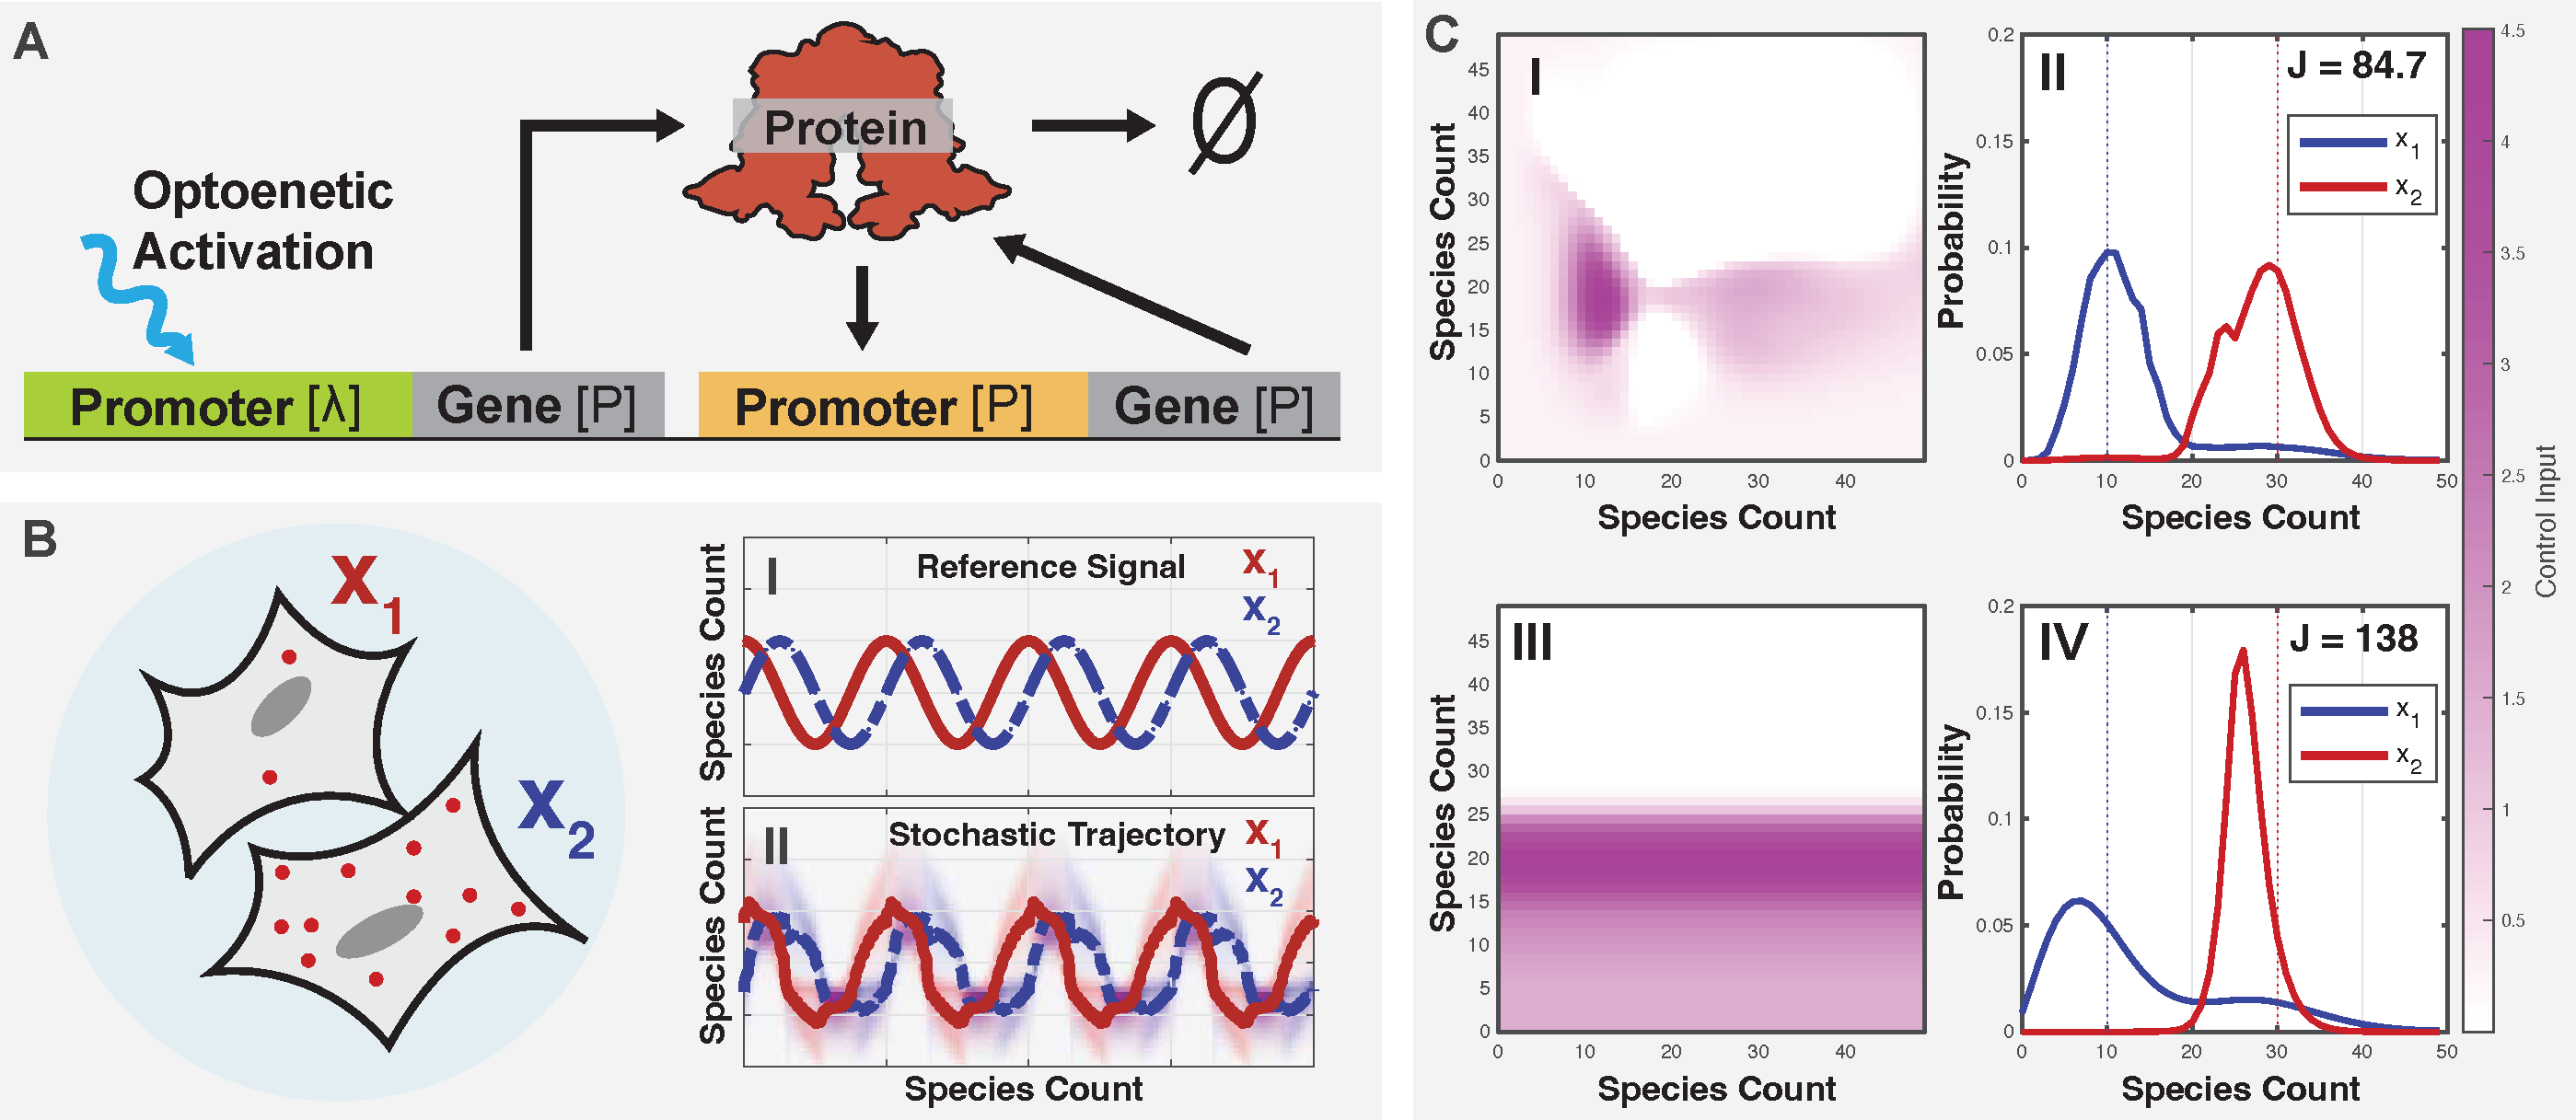
\includegraphics[width=\columnwidth]{CartoonAndControler.pdf}
\caption{{\bf Optogenetic control of multiple cells using a single light input.}
({\bf A}) Schematic of the light activated genetic system with autoregulation.
({\bf B}) Diagram of the stochastic SIMO control problem using two optogenetic cells sharing an input.
({\bf C}) Adapted from (PAPER). Noise exploiting controllers were optimized to a fully aware control input (I), and partially aware control input(III). Marginal distributions are solved using the finite state projection and show a break in symmetry using both controllers (II and IV) }
\label{cartoons}
\end{center}
\vspace{-0.3in}
\end{figure}
% XXX - Please modify figure as follows: (1) switch panels A and B to match caption. (2) Change title of panel B (previously panel A) to "External Observer, controller and actuator".  (3) Change title of panel A (previously panel B) to "Internal gene regulation pathway". (4) Change title of panel C to "Feedback control law and resulting performance"
% MMM - Made the edit

Synthetic biology seeks to create modular\cite{Ng2019} and orthogonal\cite{Liu2018} components to sense and actuate\cite{Sheets2020} complex logical systems\cite{Groseclose2020}, and which are capable of performing a variety of advanced biological behaviors\cite{Shin2020}. 
New optogenetic tools have increased our ability to actuate embedded systems within cells reliably and with strong control performance\cite{Sheets2020,Baumschlager2017,Chen2020,Lillacci2018}. Advances in these two fields have enabled computer programmable control of cellular protein production through the use of external optogenetic inputs and smart microscope techniques\cite{Fox2021,Baumschlager2021,Lugagne2017}. These types of digital-synthetic actuators allow for fine-tuned, computer-modulated control of cellular systems that were previously impossible\cite{Rullan2018, Baumschlager2017} and with fast response times in comparison to chemical diffusion. 

Classical and modern control methods like PID control and model predictive control have been implemented in such systems\cite{} which can control synthetic systems to different stable points. 
% XXX Missing Citation above.
Theoretical works have shown that stochastic systems can be controlled to unstable points by oscillating around those points \cite{Guarino2020} but new control techniques which exploit the full probability distribution information of the system can be used in certain scenarios to control simple systems to unstable points by exploiting the natural noise of protein production to its advantage. Previous control effort focus on deterministic ODE formulations of the control problem, but only a few studies seek to analyze the full chemical master equation to exploit noise to {\em improve} the control of synthetic biology processes \cite{Szymanska2015,May2021}.  

Szymanska et al.~\cite{Szymanska2015} examined a theoretical system inspired by the genetic toggle switch from Kobayashi et al.\cite{Kobayashi:2004}, where two gene products repress one another, but where degradation of one protein was under the control of UV radiation via the XXX pathway. 
% XXX - add citation to Kobayashi paper, and update name of the pathway.  I think it was the SOS pathway.
Their analysis showed that control was possible despite certain parameter errors and time delays due to maturation of fluorescent proteins and limited observation of the regulatory proteins. 
To explore this concept in the context of more realistic models and parameters, May et al.~\cite{May2021} fit a simplified stochastic model to reproduce data measured in Baumschlager, et al.\cite{} for the expression from the XXX promoter under the optogenetic control of a UV-activated T7 polymerase (see model in Figure\ \ref{cartoons}A, top promoter). 
% XXX - add details about the promoter and citation.
% XXX - let's change the order of panels A and B for this figure so that we can refer to them in the proper order.  I adjusted the text below to assume this change.
An extended model showed that addition of a positive auto-regulation module (Figure\ \ref{cartoons}A, bottom promoter) could help to maintain an elevated expression phenotype in the presence of UV excitation.
% XXX - Missing figure reference
Using discrete stochastic models based on direct solutions to the chemical master equation, it was shown that the combination of biochemical noise, nonlinear auto-regulation, and a {\em single} optogenetic feedback could allow two genetically identical cells with arbitrary initial conditions to be controlled simultaneously to reach different specified phenotypes (Figure \ref{cartoons}B). 
For example, Figure\ \ref{cartoons}C(left) reproduces the heat maps for two control laws, where the level of a single external UV excitation signal was modulated depending on the observed cellular activity, and Figure\ \ref{cartoons}C(right) shows the corresponding marginal stationary distributions that could be achieved under these control laws. 
Effective control was possible not only for a Fully Aware Feedback Controller (FAC, Figure\ \ref{cartoons}C(top)) that observed the protein counts of all observed cells, but control could be achieved nearly as well for a Partially Aware Feedback Controller (PAC, Figure\ \ref{cartoons}C(bottom)) that observed the protein counts of only one cell. 
Moreover, it was again seen that these control laws remained effective even in the circumstance where the model used to design the control law was an inexact simplification of the process dynamics to which the controller was later applied.  
%The solutions of the controllers was carried out by solving the chemical master equation (i.e., the forward Komogorov equation) to estimate the probability of possible cellular states. For a two cell, single-input-single output (SIMO) control problem, the FAC performed the best (figure\ \ref{cartoons}C(top)), and the PAC (figure\ \ref{cartoons}C(bottom)) 2nd, and pMPC controllers 3rd. In all cases, the controller's knowledge and explicit treatment of intrinsic noise was critical to improve the control performance, break symmetry, and enable the SIMO control of all cells.

In this paper, the analysis of this Single-Input-Multiple-Output (SIMO) multicellular control problem is extended to examine how the FAC and PAC controllers are affected by additional model uncertainties, including coarse grained approximations to the system dynamics, uncertainties or errors in system parameters, and delays in the biochemical sensors or optogenetic controllers through which the external feedback is implemented. In the next section, we briefly describe our methods to formulate the chemical master equation to analyze multiple individual cells in the same spatially homogeneous environment; we define the FAC and PAC controllers and their effects the dynamics of cells within that environment; and we explain how the control law is optimized to achieve desired performance objectives. Next, in the `Results' section, we explore how granularity of the model formulation, inaccuracy of parametric assumptions, or introduction of time delays would affect the FAC and PAC control performance. Finally, in `Conclusions' we summarize our findings and discuss the implications that these controllers, and their robustness to modeling errors, may have on future systems in synthetic biology.

\section{Methods}
In previous work~\cite{May2021}, a six-species gene regulation model was developed to describe light-activated association of two T7 split domains (species 1 and 2) to form active T7 polymerases (species 3) which could then in turn associate with inactive T7 promoters (species 4) to create an active gene construct (species 5) that would produce its eventual protein product (species 6). A second, far simpler single-species model was also developed by assuming quasi-steady equilibrium for the first five species. Both models were independently parametrized by fitting to the same experimental data from Baumschlager, et al.~\cite{XXX}, and then extended to include a secondary self-activated promoter-gene construct for which the expression rate was defined by a Hill function (see Eqn.\ \ref{prodRate} below). In \cite{May2021}, we showed that a control law identified using the simple model would work to achieve differential control for the more complex model, thus motivating our current study's efforts to explore further how control performance would change upon additional simplifying assumptions or errors in model specification.  In the following subsections, we discuss our methods to formulate this model, show how it is analyzed numerically, and discuss the specification of the control objective and the determination of an optimal controller.

\subsection{Model}
To examine how model approximations would affect the application of noise-enhanced control strategies, we start with the one species model from \cite{May2021} (see Fig.\ \ref{cartoons}A), which consists of two reactions: protein production and degradation.  The nonlinear light-activated protein production rate is given by
 \begin{equation}
\nu_1(x,t)= \kappa\frac{x^\eta}{x^\eta+\beta^\eta}+ k_0 + u(UV(t)),
\label{prodRate}
\end{equation}
%
%These model dynamics were then simplified to a single ODE with auto-regulation describing the protein accumulation as: 
%\begin{equation}
%\frac{dp}{dt}=u(x_1,x_2)  + \kappa\frac{p^\eta}{p^\eta+\beta^\eta}+ k_0 -\gamma p,
%\label{rateeq}
%\end{equation}
%
where $x$ is the instantaneous protein level; $\kappa$ is the maximum strength of the auto-regulation promoter; $\beta$ is the concentration at which auto-regulation promoter reaches half its strength; $\eta$ is the cooperativity in the auto-regulation promoter; $k_0$ is the promoter leakage rate; and $u(UV(t))$ is the T7 promoter strength. Through external feedback, the level of light excitation, and therefore the T7 promoter strength, $u(UV(t))$, can be modulated in response to the state of the system, thus removing explicit dependence on time. For example, in a system with the observation of two cells, one could define $u(UV(t)) = u^{\rm (FAC)}(x_1,x_2)$ as shown in Fig.\ \ref{cartoons}C(top left) for the fully aware control law, and for a system with the observation of only one cell, one could define $u^{\rm (PAC)}(UV(t)) = u(x_1)$ as shown in Fig.\ \ref{cartoons}C(bottom left) for the partially aware control law. Protein degradation is assumed to be a first order process with rate $\gamma$:
\begin{equation}
\nu_2(x) = \gamma x.
\end{equation}
Parameters describing the auto-regulation promoter, $\kappa$, $\eta$, $\beta$, and $k_0$, and the degradation rate $\gamma$
%were chosen to reproduce dynamics measured in \cite{Baumschlager2017} and 
% XXX - I don't think that this is right.  Only the parameters u(UV) and gamma were fit to data.
% MMM - yes that is right
are presented in Table 1~\cite{May2021}. 

\begin{table}[]
\caption{Model Parameters}
\begin{center}
\begin{tabular}{|c|c|c|}
\hline
Parameter & Value   & units                     \\ \hline
$\kappa$         & 0.406   & Molecules Per Minute \\
$\beta$          & 20.0    & Molecules            \\
$\eta $           & 8.00    & unit less          \\
$k_0$           & 0.0001  & Molecules per Minute \\
$\gamma$         & 0.0203  & per Minute         \\
$u$              & dynamic & Molecules per Minute \\ \hline
\end{tabular}
\label{table}
\end{center}
\vspace{-0.2in}
\end{table}

\subsection{Stochastic analyses of the model}
%Solving discrete stochastic representations of chemical dynamics is critical to the development of noise-exploiting controllers, and can be analyzed using the Stochastic Simulation Algorithm (SSA) , or the Finite State Projection (FSP).
%To recast the above ODE formulation into the discrete stochastic representation, 
To describe the discrete behavior of the above model for a population system with $N_{\rm c}$ cells, we define the current state of the system as the tuple of the non-negative numbers of proteins in each cell: $\mathbf{X}_i = [x_{1},x_{2},\ldots,x_{N_c}]_i\in \mathbb{Z}_{\ge 0}$, where the index $i$ denotes the enumeration of the state within the countably infinite set of all possible states, $\mathbf{X}_i\in\mathcal{X}=\{\mathbf{X}_1,\mathbf{X}_2,\ldots\}$.
The stoichiometry vector for a reaction in any given cell is then defined as the change in state following that reaction event (e.g., $\mathbf{X}_i \rightarrow \mathbf{X}_i + \mathbf{s}_\mu$), where the $2N_c$ possible reactions are defined in pairs corresponding to production (odd indices) and degradation (even indices) as:
\begin{align}
\mathbf{s}_1 &= \mathbf{e}_1,\ \mathbf{s}_2 = -\mathbf{e}_1,\nonumber\\ 
\mathbf{s}_3 &= \mathbf{e}_2,\ \mathbf{s}_4 = -\mathbf{e}_2,\nonumber\\
&\vdots \nonumber\\ 
\mathbf{s}_{\rm 2N_c-1} &= \mathbf{e}_{\rm N_c},\ \mathbf{s}_{\rm 2N_c} = -\mathbf{e}_{\rm N_c}, \label{Stochs}
 \end{align}
where each $\mathbf{e}_{i}\in\mathbb{Z}^{{\rm N_ c}}$ is is a Euclidean vector (i.e., unity for the $i^{\rm th}$ entry and otherwise zero). The corresponding propensity functions are:
\begin{align}
w_1(\mathbf{X}) &= u(\mathbf{X},t)  + \kappa \frac{x_1^\eta}{x_1^{\eta}+\beta^{\eta}} + k_0,\ w_2(\mathbf{X}) = \gamma x_1,\nonumber\\
w_3(\mathbf{X}) &= u(\mathbf{X},t)  + \kappa \frac{x_2^\eta}{x_2^{\eta}+\beta^{\eta}} + k_0,\ w_4(\mathbf{X}) = \gamma x_2,\nonumber\\
&\vdots \nonumber\\
w_{\rm 2N_c-1}(\mathbf{X}) &= u(\mathbf{X},t)  + \kappa \frac{x_N^\eta}{x_N^{\eta}+\beta^{\eta}} + k_0,\ w_{\rm 2N_c}(\mathbf{X}) = \gamma x_N.\label{Props}
 \end{align}


With these stoichiometry and propensities, we can formulate and run the Gillespie stochastic simulation algorithm\cite{Gillespie1992,Gillespie1977} to generate representative trajectories of the stochastic process. However, quantifying performance and designing an optimal controller requires a more direct analysis of the chemical master equation (CME).  For the same specifications of the stoichiometry and propensity functions, the CME is a linear ODE that describes how probability mass changes in time due to the specified reaction propensities and stoichiometries, which can be written:
\begin{equation}
\frac{d}{dt}P(\mathbf{X}_i)=\sum_{\mu=1}^{2{\rm N_c}}
\left(
-w_{\mu}(\mathbf{X}_i)P(\mathbf{X}_i)
+w_{\mu}(\mathbf{X}_i-\mathbf{s}_{\mu})P(\mathbf{X}_i-\mathbf{s}_{\mu})
\right).\label{CMEindex}
\end{equation}
For convenience, the CME can also be formulated more compactly in matrix/vector form as:
\begin{equation}
\frac{d}{dt}\mathbf{P}=(\mathbf{A}_0+\textbf{Bu}^{\mathcal{C}})\mathbf{P},\label{CME}
\end{equation}
where $\mathbf{P} = [P(\mathbf{X}_1), P(\mathbf{X}_2), \ldots ]^T$ is the enumerated probability mass vector for all possible states of the system; $\mathbf{A}_0$ is the infinitesimal generator of the stochastic process due to the autoregulation promoter and degradation events;  $\textbf{u}^{\mathcal{C}} =[u^{\mathcal{C}}(\mathbf{X}_1), u^{\mathcal{C}}(\mathbf{X}_2), \ldots ]^T$ is the collection of control inputs associated with each state; and $\textbf{Bu}^{\mathcal{C}}$ is the contribution that these control inputs make to the infinitesimal generator when included into the feedback process. 
 
More specifically, the open-loop infinitesimal generator, $\mathbf{A}_0$, is constructed according to:
\begin{equation}
[\mathbf{A}_0]_{ij} = \left\{
\begin{array}{rl}
-\sum_{\mu =1}^{2N_{\rm c}} w_{\mu}(\mathbf{X}_j), &\text{for }i=j,\\
w_{\mu}(\mathbf{X}_j), &\text{for }\mathbf{X}_i = \mathbf{X}_j+\mathbf{s}_\mu\\
0, & \text{otherwise,}
\end{array}\right. 
\label{InfA}
\end{equation}
and the feedback infinitesimal generator, $\mathbf{Bu}^{\mathcal{C}}$, of the controller is constructed according to
\begin{equation}
[\mathbf{Bu^{\mathcal{C}}]}_{ij} = \left\{
\begin{array}{rl}
- N_{\rm c}{u}^{\mathcal{C}}(\mathbf{X}_j), &\text{for }i=j\\
{u}^{\mathcal{C}}(\mathbf{X}_j), &\text{for }\begin{array}{ll}\mathbf{X}_i =\mathbf{X}_j + \mathbf{e}_{i_{\rm c}}, \\ \text{and } i_{\rm c} = 1,\ldots,N_{\rm c}\end{array},\\
0, & \text{otherwise,}
\end{array}\right.
\label{InfB}
\end{equation}
where ${u}^{\mathcal{C}}(\mathbf{X}_j)$ is the specification of the $\mathcal{C}$ controller in terms of the state, or its partial observations.

For a given controller, the equilibrium distribution of the system ($\mathbf{P}^*$) can be found by solving Eq.\ \ref{CME} and is given by:
\begin{equation}
\mathbf{P}^*={\rm null}(\mathbf{A}+\textbf{Bu}^{\mathcal{C}}).\label{SSDist}
\end{equation}


\subsection{Quantification and optimization of control performance}
%To quantify the performance of the controlled system, Score metrics of steady state distributions were made in order to enable optimization of the system by adjusting controllers.

For the single-input-multiple-output control of the multiple cell system, any input signal that is applied to one cell in the population will be felt by all cells in the population. As a result, it is not possible to independently control any individual cell without introducing changes to the behavior of the others. Therefore, an effective controller must be able to strike a balance among the desired behaviors of all cells in the system.

To quantify performance success, we define the performance error score, $J$, as the expected steady state squared Euclidean distance of the process from the specified target state, $\mathbf{T}$:
 \begin{equation}
 J = E\{(\mathbf{X}-\mathbf{T})^2\}.
 \end{equation}
This score is easily calculated by applying a linear operation on steady state probability distribution $\mathbf{P}^*$ from Eq.\ \ref{SSDist}) as follows:
{ \begin{align}
J&= \lim_{t\rightarrow \infty}\mathbb{E}\{|\mathbf{X}(t)-\mathbf{T}|_2^2\}, \nonumber \\ 
&=\sum_{i_1,i_2,\ldots} P^*(x_1=i_1,x_2=i_2,\ldots) \left[(i-\mathbf T_1)^2 + (j-\mathbf T_2)^2 +\ldots\right],\nonumber  \\
&=\sum_{i,j,\ldots} P^*_{ij\ldots}(t)C_{ij\ldots} =\mathbf{C}\mathbf{P}^*,
\label{Euclid}
\end{align}} where $\mathbf{C}$ is simply a vector that contains the squared Euclidian distance of each state from the specified target T, i.e., $C_i = |\mathbf{X}_i-\mathbf{T}|_2^2$. As a result of this calculation, $J$ is a non-negative scalar that is zero if any only if $\mathbf{P}^*$ is a delta distribution located exactly at the target vector $\mathbf{T}$.

In this work, we explore two different controller designs that allow for the controller to use two different types of information. A fully aware controller ($\mathbf{u}^{FAC}$) uses direct observation of the protein count of two cells simultaneously while making its control input decision, while the partially aware controller $\mathbf{u}^{PAC}$) uses only the direct observation of a single cell:
\begin{equation}
\mathbf{u}^{FAC}=u(x_1,x_2)
\end{equation}
\begin{equation}
\mathbf{u}^{PAC}=u(x_1)
\end{equation}
% XXX - Do we need to use 0 and 1.  Why not use 1 and 2 so that this can match better to the formulaton above?  I changed them to x1 and x2 here, but please chekc to make sure that this is sonsistent throughout text and figures.
% MMM - Made the change to x1 x2
where $x_1$ and $x_2$ are discrete integers greater than or equal to zero that represent the number of proteins in cell one and cell two. In \cite{May2021}, the controllers $\mathbf{u}^{FAC}$ and $\mathbf{u}^{PAC}$ controllers were optimized to minimize $J$, and both $\mathbf{u}^{FAC}$ and $\mathbf{u}^{PAC}$ were saved as lookup tables after being optimized. In what follows, we will use these controllers exactly and without modification to explore how performance changes when the controllers are applied to systems that are approximations of the model under they were originally designed.

\subsection{Scaling for system granularity}
One of the major computational obstacles in using the CME or FSP formulations to analyze discrete stochastic chemical kinetics is that the dimension of the FSP scales linearly with each chemical species, and therefore exponentially with the number of independent species. To circumvent this issue, several previous studies have projected the FSP onto lower dimensional spaces based using various techniques such as time scale separations\cite{Peles2006}, Krylov subspaces\cite{Macnemara&Sidje?}, coarse meshes\cite{Munsky2008IEEE,Tapia2012CDC}, or principle orthogonal decompositions\cite{Vo2019}.
% XXX - would be good to look for a few other examples outside of our own papers where the CME dimension is reduced by linear projections.
On the other hand, an experimental obstacle to using CME analyses is that gene expression quantification based on fluorescence intensities (e.g., using fluorescent protein reporters) usually does not provide molecular resolution, but rather measures only relative changes in expression over time.

To address how variations in model or observation scales might impact the effectiveness of noise-based control, we use the controller optimized at one resolution and ask how effective it would be when applied to systems with the same dynamics but with different resolution. 
To accomplish this rescaling, let $M$ denote some metric for the size of the original system (e.g., the average number of proteins at steady state and maximal UV) and let $M'$ denote the same metric for the system at a different resolution.  
Toward this goal, we define a granularity parameter ($\alpha=M'/M$) that linearly scales the species populations to increase ($\alpha>1$) or decrease ($\alpha<1$) the maximum populations size, while maintaining the dynamics and general behavior of the model. To apply the granularity parameter, we assume that each propensity function, $w_{\mu}$, from Eqns.\ \ref{Props} is rescaled to a different level of discreteness by substituting
\begin{equation}
w'(\mathbf{X})=w(\mathbf{X}/\alpha).
\end{equation}
For example, the production and degradation of protein in cell one would become:
\begin{equation}
w'_1(\mathbf{X}) = u(\mathbf{X}/\alpha,t)  + \kappa \frac{(x_1/\alpha)^\eta}{(x_1/\alpha)^{\eta}+\beta^{\eta}} + k_0,\ w'_2(\mathbf{X}) = \gamma x_1/\alpha.
\end{equation}
% XXX - Please check this against what you did computationally. 
After this rescaling, if $\alpha<1 $ the system dynamics will now occur over a smaller range of protein counts, and if $\alpha >1$ the system dynamics occurs over a larger range of protein counts. 

We note that in transforming the propensity functions, the inputs to the controller have also be scaled by $1/\alpha$ before computing the appropriate functions of that state, e.g., ${u}^{\mathcal{C}} = {u}^{\mathcal{C}}(\mathbf{X}/\alpha)$. Because identification of the original control formulation, $\mathbf{u}^{FAC}(x_1,x_2)$ and $\mathbf{u}^{PAC}(x_1)$ only considered integer values for $(x_1,x_2)$, fractional number inputs for after rescaling $(x_1/\alpha,x_2/\alpha)$ are handled by 2D cubic interpolation of the nearest values.
%\begin{equation}
%u'=u(x_0 / \alpha, x_1 / \alpha) 
%\end{equation}
%\begin{equation}
%u'=u(\alpha x_0)
%\end{equation}
Finally, to provide a consistency relative scoring, the definition of the performance score is also adjusted according to sale magnitudes, i.e.,:
{\begin{align}
J' &= \sum_{i=0}^{M'}  \sum_{j=0}^{M'}P^*(x_1=i,x_2=j) ((i/\alpha - \mathbf T_1)^2 + (j/\alpha -\mathbf T_2)^2),\nonumber \\
& =\mathbf{C}'\mathbf{P}^*
\label{EuclidV}
\end{align}}

\subsection{Observation and actuation time delays}
No real optogenetic control system can provide instantaneous feedback -- there will always be delays in biochemical reactions needed for observations (e.g., transcription and translation dynamics as well as folding and maturation of fluorescent proteins), delays in data analysis and decision making (e.g., image processing and calculation of the corresponding control signals), and delays in the actuation dynamics (e.g., activation of optogenetically excitable molecules).  To explore the impacts of delays between the time a cellular fluctuation occurs and the time at which the corresponding control action can take effect, we developed a simple time-delay stochastic simulation algorithm. In this analysis, the state history is recorded following every stochastic event, allowing for reconstruction of the piecewise constant history of the species' populations, e.g., $x_1(s)$ and $x_2(s)$ for all $s\in [0,t]$.  Using this information, the time-delayed control signal at time $t$ can be specified as: 
\begin{equation}
u_{\tau}(t)=\left\{
\begin{array}{rl}
      0 ,&\text{ for }  t \leq \tau, \\
      {u}^{\mathcal{C}}(x_1(t-\tau), x_2(t-\tau)) , &\text{ for }   t > \tau,\\
\end{array}\right. 
\label{timeDelaySSA}
\end{equation}
where $\tau$ is the time delay between observation and actuation, and ${u}^{\mathcal{C}}$ is the previously optimized control law (e.g., $\mathbf{u}^{\rm FAC}$ or $\mathbf{u}^{\rm PAC}$). We note that the time delay stochastic process was only simulated using the SSA because to our knowledge an appropriate direct FSP/CME integration procedure has not yet been developed.

%\subsection{Parameter Scalings and Sensitivity}
%Finally, to explore the sensitivity of the control performance to inaccuracies in model parameters for one or more cells, we calculate the control performance score ($J$), over a range for each parameter scaled linearly with a scaling parameter ($\zeta$) while holding all other parameters constant. 
%%Any new arbitrary parameter $\lambda\in \{ \kappa,\beta,k_0,\eta,\gamma\}$ can be rescaled from an old one ($\lambda$) according to
%%\begin{equation}
%%\lambda' = s \lambda
%%\end{equation}
%We explore two types of sensitivity analysis: one which performs the analysis on one cell at a time while keeping the other constant, and another which scales similar parameters in both cells at the same time. 
%%In the former case, it should be noted that each cell receives its own set of parameters, so that the number of parameters double during sensitivity analysis of a two cell control process. 
%In either case, steady state distributions of the perturbed models are solved using the FSP.
% XXX - I don't think that we need this section in Methods -- but perhaps some of the text should be moved to the results if needed.

\section{Results}

\subsection{Effects of Parameter Errors or Extrinsic Uncertainties}
\begin{figure*}
\begin{center}
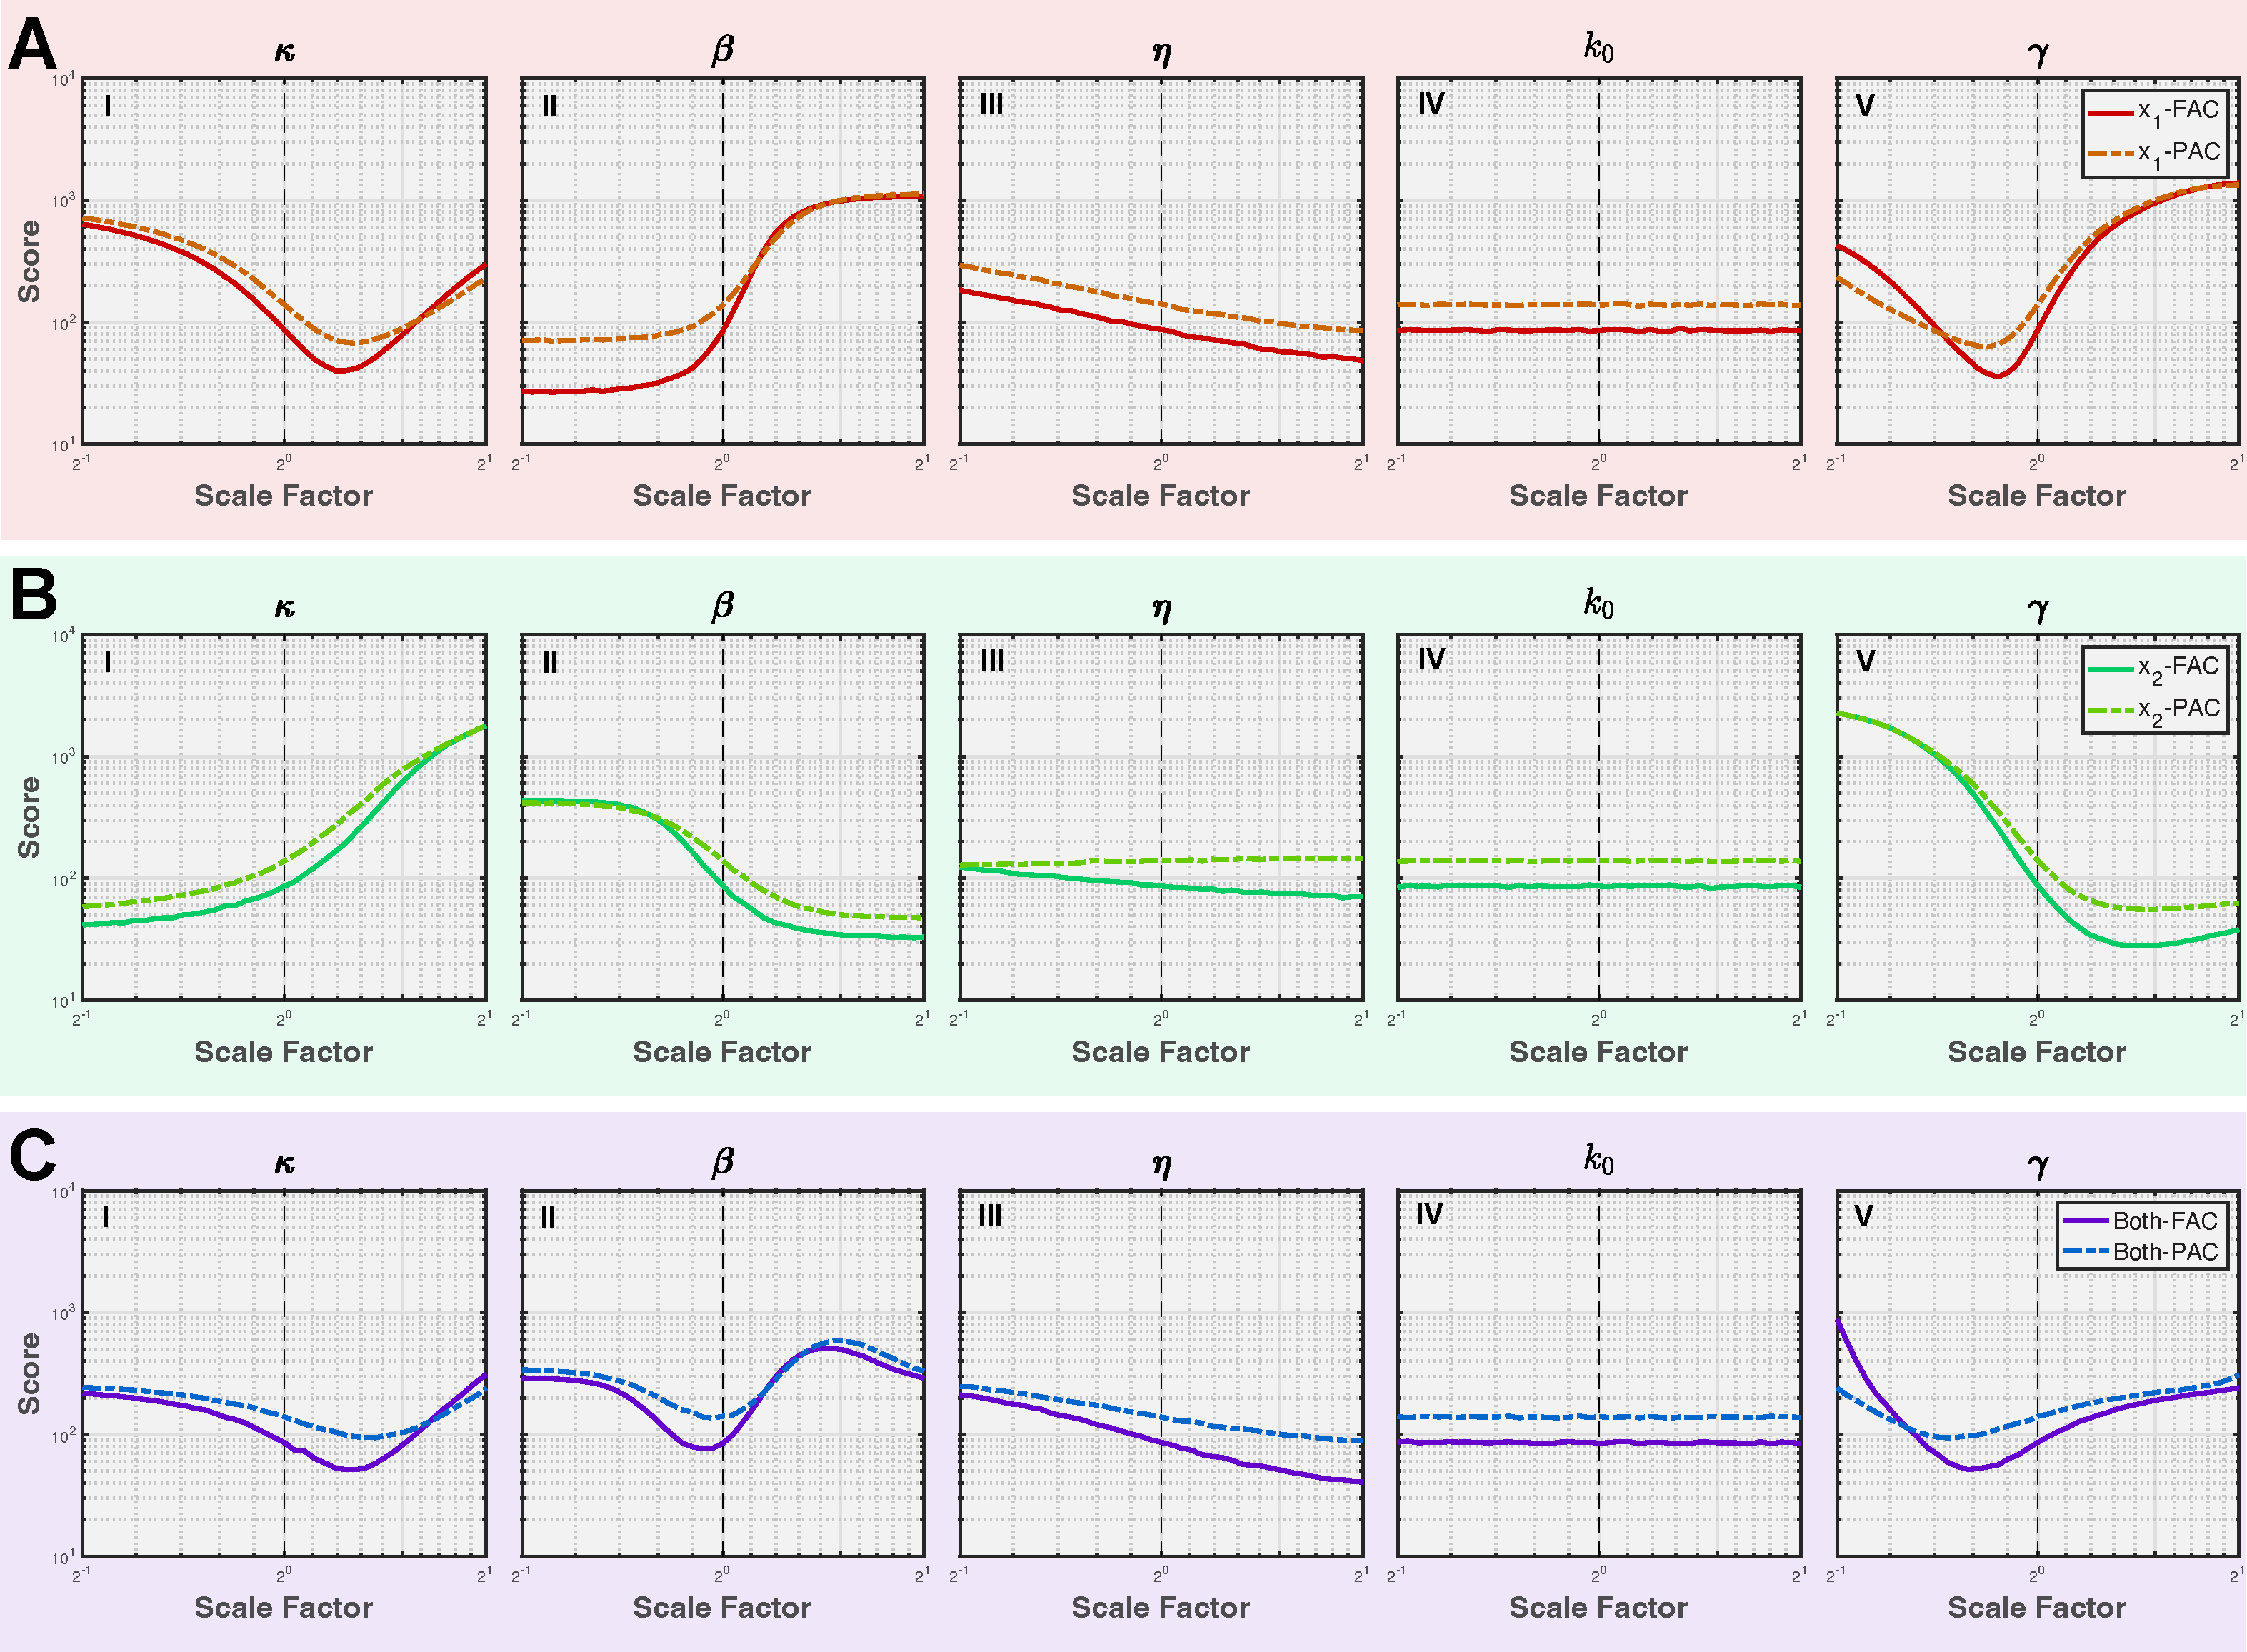
\includegraphics[width=1\textwidth]{ParameterPerturbation.pdf}
\caption{Parameter sweeps using the FAC and PAC show a broad range of control performance in cell 1 ({\bf A}),  in cell 2 ({\bf B}), and in both cells ({\bf C}). }
\label{Parameter}
\end{center}
\end{figure*}

Exact parameters values are typically unknown for real stochastic process, and even genetically identical single-cell systems can exhibit cell-to-cell heterogeneity in parameters due to extrinsic variations outside of the specific pathways of interest. Estimates of parameters can be taken, but not exact measurement. These parameter uncertainties could influence system performance. To explore the sensitivity of control performance to unknown errors in the model parameters, sensitivity analysis was performed for each model parameter and for the situation where the corresponding parameter was modified in either one cell at a time (i.e., to simulate extrinsic noise) or in both cells simultaneously (i.e., to simulate parameter errors).  For each perturbation analysis, both the $\mathbf{u}^{\rm FAC}$ and $\mathbf{u}^{\rm PAC}$ controller were analyzed over a range of parameters from one-half to two-fold of the original parameters.
% XXX - How hard would it be to extend this to 10 fold in either direction?
% MMM-Changes to parameters can dramatically change the location of the probability distribution which is contained in a bounded (50,50) area. A 10 fold increase to a parameter can push all the probability to the top corner of the space
 Figure \ref{Parameter}A shows the results for these parameter sweeps when a single parameter in Cell 1 is change while the parameters of Cell 2 is held fixed, and Fig.\ \ref{Parameter}B shows the opposite when changes Cell 1 has fixed parameters and Cell 2 is modified.  Finally, \ref{Parameter}B  shows the performance change when the corresponding parameter is changed in both Cell 1 and Cell 2 at the same time.
 
Modification to parameters was found to produce a broad range of effects, where some changes increase performance, some decrease performance, and others have little or no effect. For example, increasing $\beta$ in Cell 1 worsens performance while increasing $\beta$ in Cell 2 improves performance (compare second column in Fig.\ \ref{Parameter}A and \ref{Parameter}B). In some cases, these effects were not monotonic; for example, increasing $\kappa$ in Cell 1 (Fig.\ \ref{Parameter}A, left column) would be highly advantageous up to a limit after which the control performance degrades rapidly. In other cases (such as for $k_0$), the effect of parameter perturbations on performance is insignificant even for relatively large ($s$=2) perturbations.Similarly, Fig.\ \ref{Parameter}C shows that when parameters of both Cell 1 and Cell 2 are jointly changed, these changes could also improve or detract from control performance.
%It was found that the $\mathbf{u}^{\rm FAC}$ often outperformed the $\mathbf{u}^{\rm PAC}$, but for large $s$ in a few parameters the inverse was found (figure \ref{parameter} (Row III, E and At).

When examining the effects of changing parameters when using the $\mathbf{u}^{\rm FAC}$ (solid lines) or the $\mathbf{u}^{\rm PAC}$ (dashed lines), general trends typically remained the same in that changes to a parameter which cause a decrease in the control performance of the FAC also tend to decrease the performance of the PAC. Some parameters (e.g., $\kappa$, $\gamma$) reached minima that performed better than the original, which suggests that the physical system itself has room for optimization beyond the original design that could lead to better control performance, {\em even without changing the control law}.  One explanation for why changes to $k_0$ had no effect on control performance is that the original parameter was so small that it may require a larger scaling on a different magnitude before changes are observed. 
% XXX - what is \eta?  From the table this should be the cooperativity with is very large.  Is this a mistake?
% MMM - This was k_0, not eta
In a few circumstances, changes in the parameters $\kappa$ or $\gamma$ led to the surprising situation where the PAC controller, which only observes one cell at a time, was more robust to parameter errors than was the FAC controller, which can observe both cells, even to the extent that the PAC controller could sometimes outperform the FAC.  We stress that this effect is due to the mismatch between the assumed and the actual parameters, and re-optimizing the two controllers for the new parameter combination will always yield better control results for the FAC compared to the PAC.


To assess the potential robustness of noise-enhanced control of the proposed synthetic auto-repression toggle switch, we adopted the model  from \cite{May2021} as well as the fully aware and partially aware controllers, $u^{\rm FAC}(x_1,x_2)$ and  $u^{\rm FAC}(x_1)$, respectively as described in the methods section.  In the following subsections, we explore how well these controllers would perform in the more realistic setting where the approximate model used to define the controller no longer matches exactly to the dynamics of the process that the controller is being used to manipulate. 

We first explore how the model defined for a given assumed system size (i.e., in which protein numbers have a range of $M$) when applied to a system with larger or smaller systems sizes (i.e., where protein numbers now have a range of $M' = \alpha M$.  This modification could arise from two situations related to numerical convenience or inexact resolution in the measurement of concentrations. First, from the perspective of numerical convenience when optimizing a controller, it can be advantageous to reduce the assumed range of protein levels in order to reduce the dimension of the CME and FSP analyses, thereby achieving a more tractable optimization problem.  For example, the current model (see Methods) takes 19.3 seconds to solve the FSP analysis when $\alpha=1$ but the same analysis takes 24619 seconds to solve when $\alpha=10$. Since numerical optimization of the controller can take many millions of calculation for different control laws, learning a controller using $\alpha=1$ that works for $\alpha=10$ would yield substantial savings in computational effort. The second situation under which sensitivity to system scaling could become important is when measurements are relative and do not provide single-molecule resolution. For example, in measurements like those on \cite{Baumschlager} which are based on fluorescence protein intensities, it is not clear how many proteins correspond to what level of fluorescence intensity, and the scalar $\alpha$ is an unknown quantity that must be estimated (e.g., through calibration with single-molecule measurements or dilution experiment\cite{XXX - look for elowitz paper or something similar that tried to calibrate for single-molecule counts}). 
% MMM - Ding:2019??
It is well established that the relative size of stochastic fluctuations (i.e., noise) in a chemical process decreases with the inverse square root of the process scale \cite{Kampen1961}. As the system size increases (with all species being scaled by the same factor), the dynamics approach those of a deterministic process with probability one (with zero-measure exceptions only for initial conditions lying on manifolds that separate attractors for different steady state behaviors)\cite{XXX}. For the purpose of noise-induced control, this introduces a tradeoff where noise is critical to break symmetry and enable differential control, yet noise is also deleterious to maintaining desired states once they have been achieved. Considering these competing objectives, it is not immediately clear how the reduction of noise through the addition of system granularity will affect control performance. 

To shed light on this tradeoff, control performance scores for the $\mathbf{u}^{\rm FAC}$ and $\mathbf{u}^{\rm PAC}$ controllers were calculated at different levels of granularity ($\alpha$) between 0.1 and 2.0. 
% XXX - Why only go up to 2?  Did it become intractable?
% MMM - Non_Sparse Calculations are intractible after 2, but sparse versions of code will work fine
Figure \ref{Volume} (Ai - Fi) shows the joint (left plots) and marginal (right plots) distributions of the two cells relative to the specified target position (circles in joint distributions and vertical dashed lines in marginal distributions) for the FAC controller and for $\mathbf{\alpha}$=.2 (A,B), 1 (C,D) and 2 (E,F). As the granularity changes from $\alpha$=0.2 , to $\alpha$=2, the distributions become focused at a point near the target, and the performance score improves from $J=$333 to 85 to 27, respectively. The PAC controller performance also improves considerably with alpha as shown in Fig.\ \ref{Volume} (G-L).
% XXX - Please change the panel labels to A-F, G-L, and M.
% MMM - made the change
\subsection{Effects of changes to system granularity}
\begin{figure*}[t!]
\begin{center}
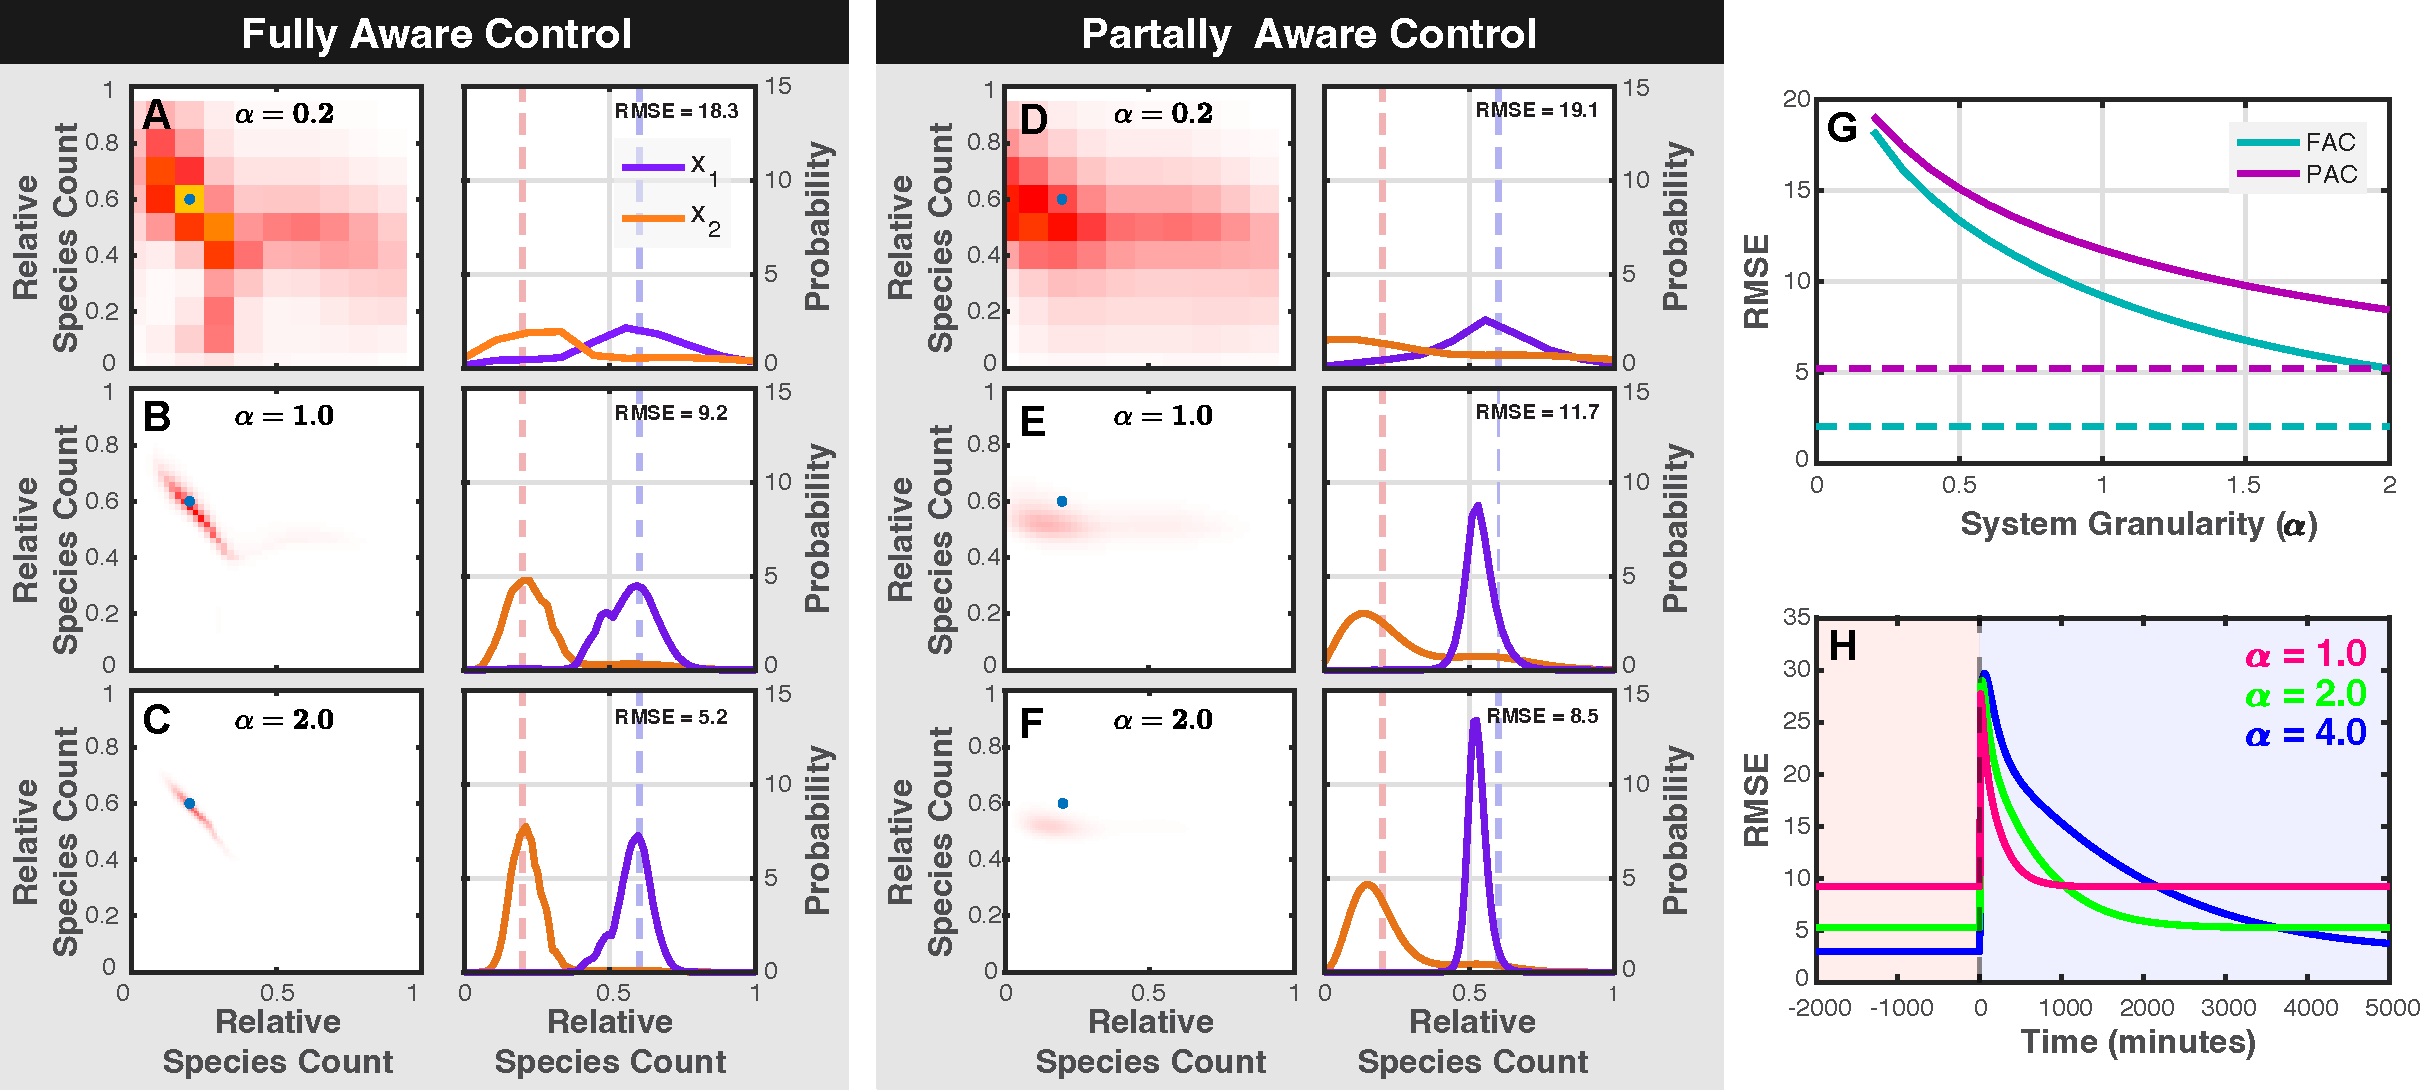
\includegraphics[width=1\textwidth]{GranularityPerturbation.pdf}
\vspace{-0.1in}
\caption{Systems with high granularity were shown to have increased control performance but slower response times.}
\label{Volume}
\end{center}
\vspace{-0.2in}
\end{figure*}
% XXX - This figure needs larger fonts for all the labels and axes. 
% MMM - made the change
% Update panel letters as written in caption
% Add tic marks to left side of the A and C heat maps

Figure \ref{Volume}M shows the trend of the performance score versus alpha for both the FAC (solid cyan line) and the PAC (solid magenta line) controller. This improvement in performance appears to approach a small value as the granularity goes to infinity, but since the size of the FSP increases with the square of the system size, systems much larger than $\alpha$=2 (where $\mathbf{A}_0\in \mathbb{R}^{10^4\times10^4}$) become more difficult to calculate. 
% XXX - I would think you should be able to compute larger values of 10^6.  They would be slow, but should be doable in a few minutes per calculation.
% MMM - constructing the FSP takes longer than solving it
To bypass this limit in the FSP, sixteen SSA simulations were used to sample the CME of a system with a much larger volume of $\alpha$=100. Each SSA was ran for $5\times10^7$ minutes and only the last $4\times10^7$ minutes were sampled to estimate the stationary distribution and the calculate the performance score. The performance score estimates of this high granularity SSA using the FAC and PAC were 4.13 and 27.5 respectively, which are plotted as dashed lines in Fig.\ \ref{Volume}G. Although it is unclear if further performance improvements could be obtained with further increases to the system scale, for all cases considered so far, we found that both controllers monotonically improved with increased $\alpha$ and that $\mathbf{u}^{\rm FAC}$ always outperforms the $\mathbf{u}^{\rm PAC}$. 




We note however, that the improved steady state performance for systems with larger scales, comes at a cost that they also take longer to reach a steady state distribution. This tradeoff is illustrated in Fig.\ \ref{Score} which shows the performance score $J(t)$ as the system adapts to a change from the original target point $\mathbf{T} = [30,10]$ to its mirror point $\mathbf{T}_m = [10,30]$.  
% XXX - Please add a new figure to show this point.  Start with an initial condition that is the steady state with target T and then flip it to T' = T(::-1).  Then solve for P(t) and calculated J(t) from this.    Finally, make a plot of J(t) versus t for the three cases \alpha = 0.2, 1, 2.
One hundred SSA simulations of the flip-mirroring process were simulated while measuring the average score all simulations over time. Fig.\ \ref{Score} (A and B) shows the average score and protein counts of the simulation when $\alpha=1$, Fig. \ \ref{Score} (C,D) when $\alpha = 10$, and Fig. \ \ref{Score} (E,F) when $\alpha = 100$. 

From the figures it is clear that the smaller $\alpha$ creates faster dynamic but also have higher scores due to inherit noise. When $\alpha = 10$, the system becomes much less noisy and have lower scores but takes some time to respond. When $\alpha$ is too large at 10, the system contains very small levels of noise, but the dynamics
 % XXX - update this to explain what you see in this new figure. 

%These data suggest that increasing granularity increases steady state control performance even if the controller itself depends on noise for its implementation. Also, designing a controller to work for a system of one volume size can result in a controller that works even for another much larger volume.  This has practical significance, because it is relatively easy to search over a control law defined on a small $M\times M$ grid of states (e.g., when $M$=50 as in \cite{May2021}), but to implement the controller for a larger system which may be computationally prohibitive. This result implies that it may be possible to optimize controller using coarse-grained FSP analyses for small granularity problems and adapt these via interpolation for use with larger, more realistic systems, that exceed the computational limit of standard FSP computations.  

\subsection{Effects of Time Delays on Controller Performance}
\begin{figure*}
\begin{center}
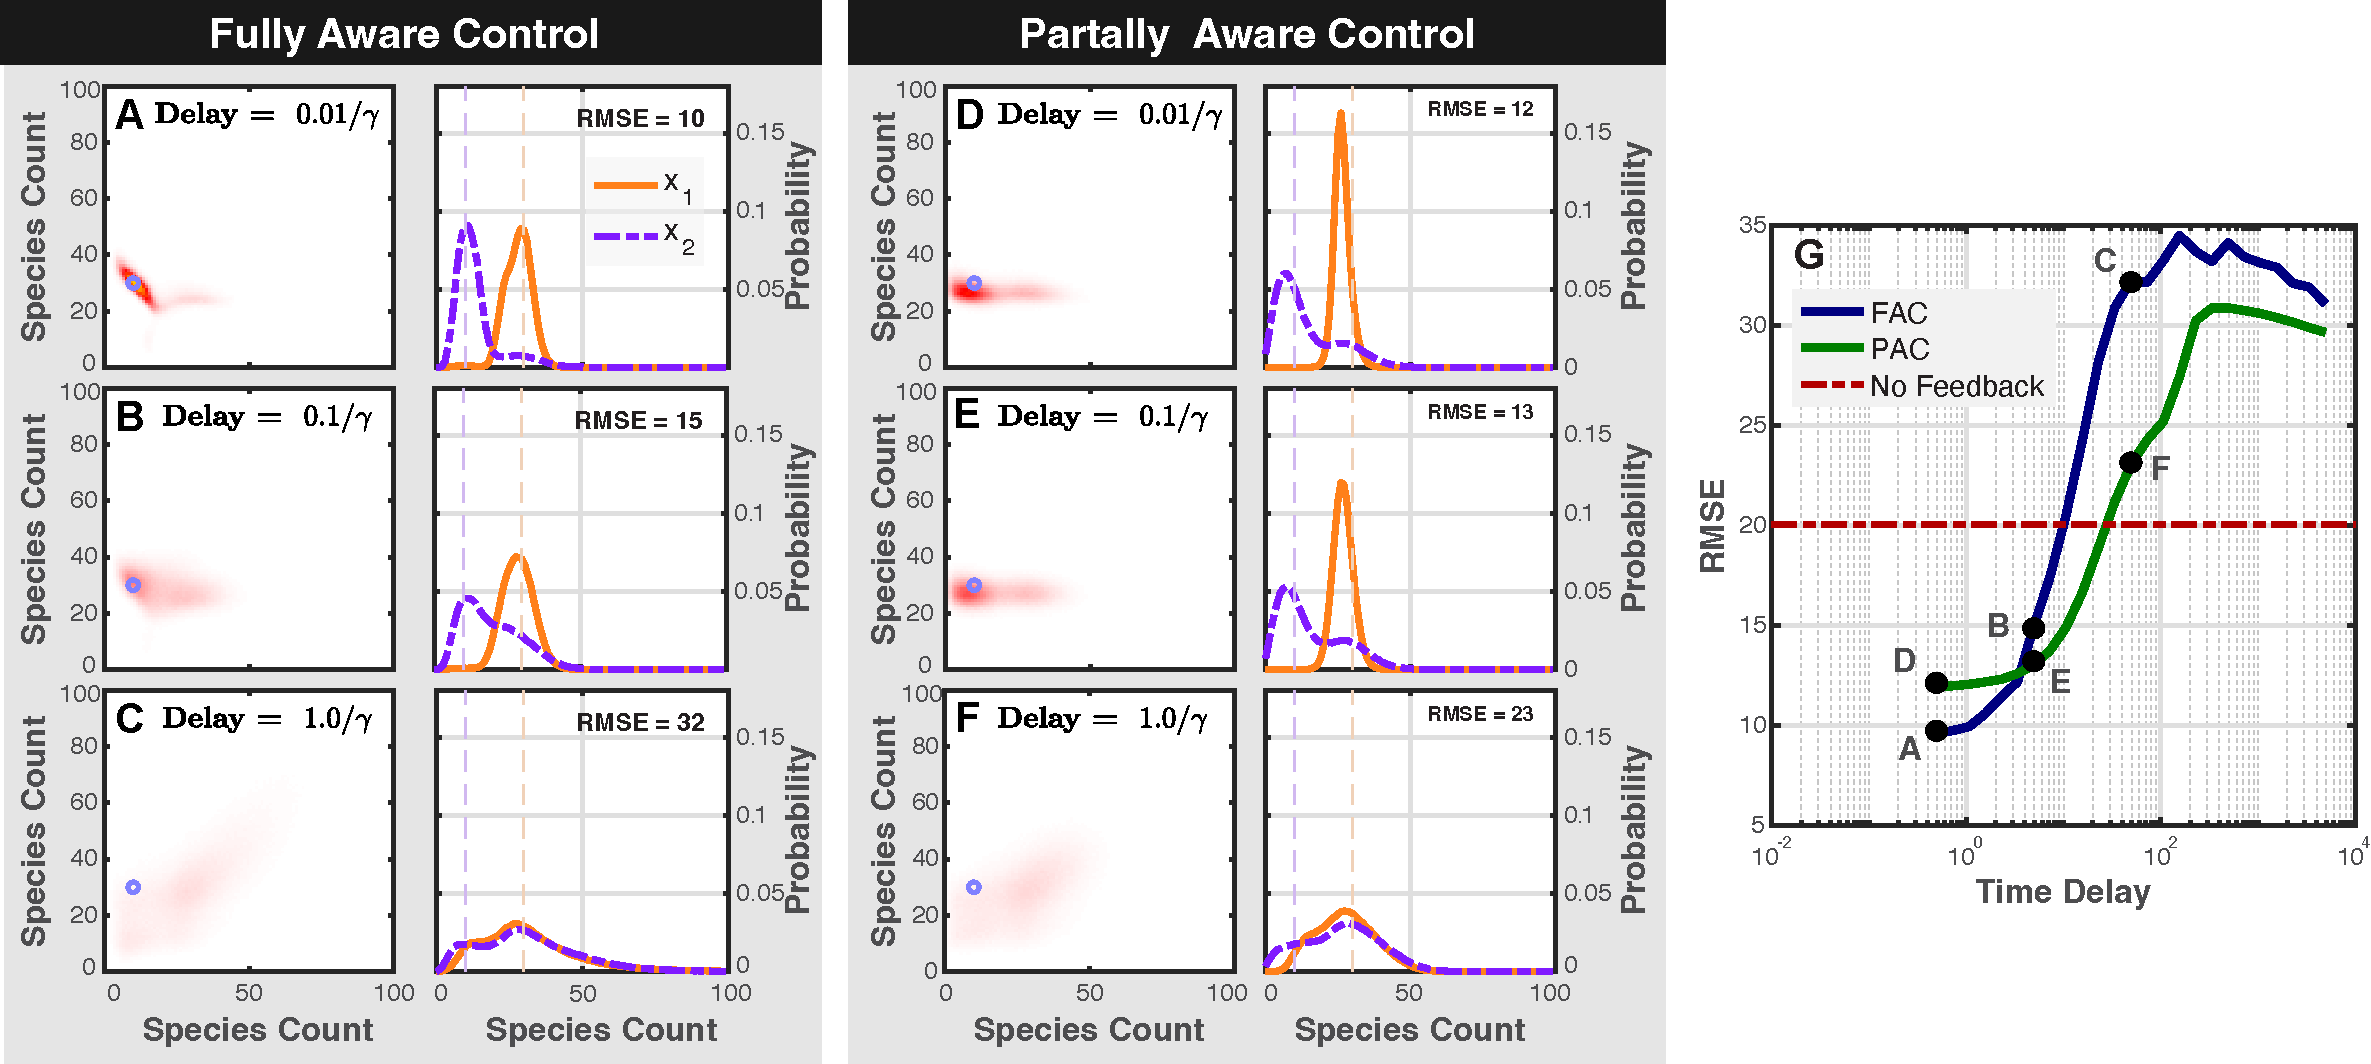
\includegraphics[width=1\textwidth]{TimeDelayPerturbation.pdf}
\vspace{-0.1in}
\caption{Stochastic simulations of the time delayed system show decreasing control performance using either controller. }
\label{Time}
\end{center}
\vspace{-0.2in}
\end{figure*}
% XXX - This figure needs larger fonts for all the labels and axes. 
% MMM- Did the change
% Update panel letters as written in caption
% Add tic marks to left side of the A and C heat maps
% Fix the ref to baumschlager paper.

Feedback control can only be effective if one can quickly make measurements, compute adjustment to the control signal, and implement the needed change to the system. As the time required for any of these steps increases, control performance will be degraded, perhaps even leading to large fluctuations or instability. To explore how time delays would affect the noise-enhance controller $\mathbf{u}^{\rm FAC}$ and $\mathbf{u}^{\rm PAC}$, we generated large sets of time-delayed stochastic simulations (see Methods) for different lengths of the time delay. Each SSA was sub-sampled for 1000 times over 10000 minutes of simulation time after a burnin period of 10000 minutes.

Figure \ref{Time} shows the joint and marginal distribution of each controller and time-delay pair and the resulting score, with panels A-F showing results for the FAC controller and panels G-L showing results for the PAC controller. Figure \ref{Time}M summarizes these results by plotting the score of both controllers versus the time delay. From the figures, it is clear that performance is rapidly degraded as the delay approaches and then exceeds the characteristic time scale of the process. At very small time delays (below $\tau = 0.07/\gamma = 0.0142$ min), the FAC outperforms the PAC ($J=$87 versus 146 at $\tau = 0.01/\gamma = 0.00203$ min) but at moderate time delays (above $\tau = 0.07/\gamma = 0.0142$ min) the PAC outperforms the FAC ($J=$170 versus 219 at $\tau = 0.1/\gamma = 0.0203$ min). 
% XXX - you can use the value of gamma=0.203 in Table 1 to write these in units of minutes.

This data taken together show that time much larger that $0.07 / \gamma = 0.0142 min$ is detrimental to the FAC controller; delays beyond $0.2 / \gamma = 0.0406 min$ are detrimental for the PAC controller; and the best choice in controller is dependent the level of time delay in the system.  For extreme levels of time delay, both systems lose their asymmetry, and their scores become much worse ($J=$1041 and 931). A no-feedback controller was developed which required no inputs. Such a controller is immune to time delay, and received a score $J=402$. These data show that at large time delays above , attempting to improve control with feedback is worse than no-feedback.

% XXX - This figure needs much larger fonts for all the labels and axes.
% MMM - Did the change
% There are errors in the parameter names.  What is 'alpha'?
% remove the A,B,C,D,E.
% replace I, II, III with A, B, C
% what is parameter $\mu$? Is that an error?  Please use $\mu$ for reaction index as in the methods section.

\begin{figure*}
\begin{center}
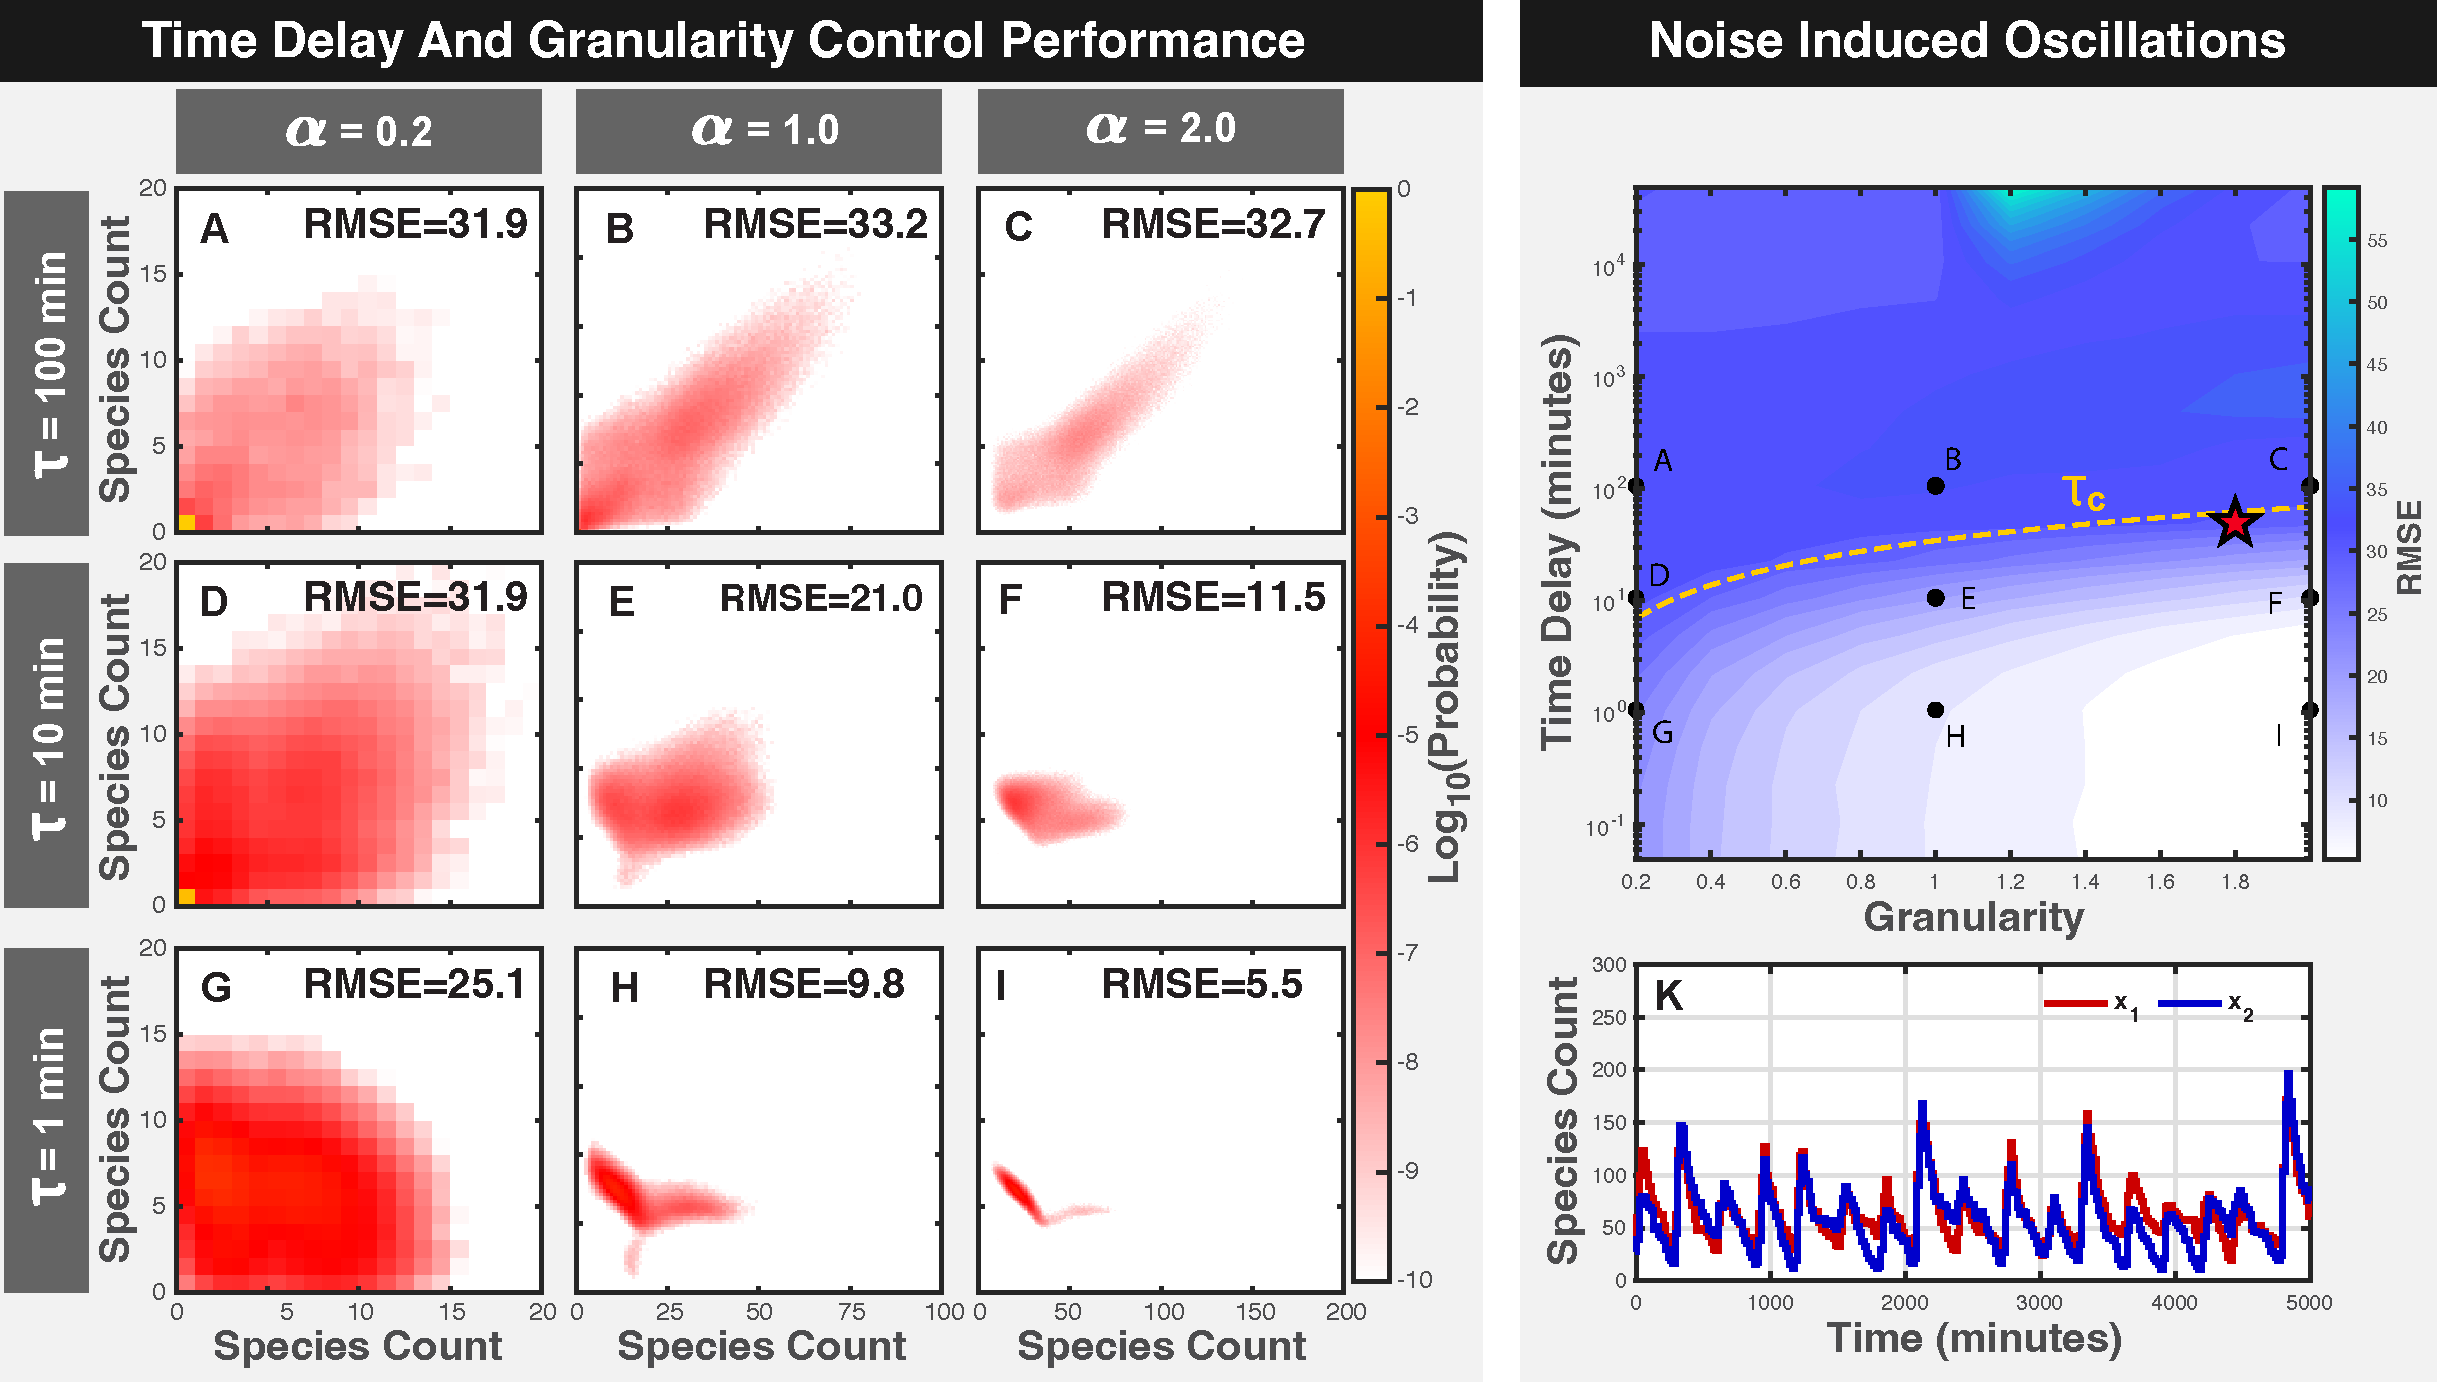
\includegraphics[width=1\textwidth]{DelayAndGranularity.pdf}
\vspace{-0.1in}
\caption{Stochastic simulations of the FAC driven system (A) and PAC driven system (B) show different failure modes at at different $(\tau,\alpha)$ pairs (C).}
\label{DG}
\end{center}
\vspace{-0.2in}
\end{figure*}

Joint analysis of time delay and granularity together was performed to better understand if granularity can undo the effect of time delay. System control performance was analyzed over a two dimensional domain of points $(\tau,\alpha)$ using sixteen stochastic simulations for XXX minutes. These simulations were driven using the FAC controller Fig \ref{DG} (A), and PAC controller Fig \ref{DG} (B). The landscape of the FAC and PAC control performance Fig \ref {CtrlP}(A and B)over the domain shows a valley at low $\tau$, and a plateau at large $\tau$. This suggests that increasing system scale at large time delays is not beneficial to control performance. To better understand the appearance of the landscape, trajectories in different regions were compared. Trajectories at the edge of the plateau region (blue star) showed bursty behavior Fig \ref {CtrlP}(C)(blue lines), while trajectories at the edge of the valley Fig \ref {CtrlP}(C) (red lines) showed oscillatory behavior. Despite the small different in time delay between the red and blue trajectory, a stark change to the overall behavior was observed.

\begin{figure*}
\begin{center}
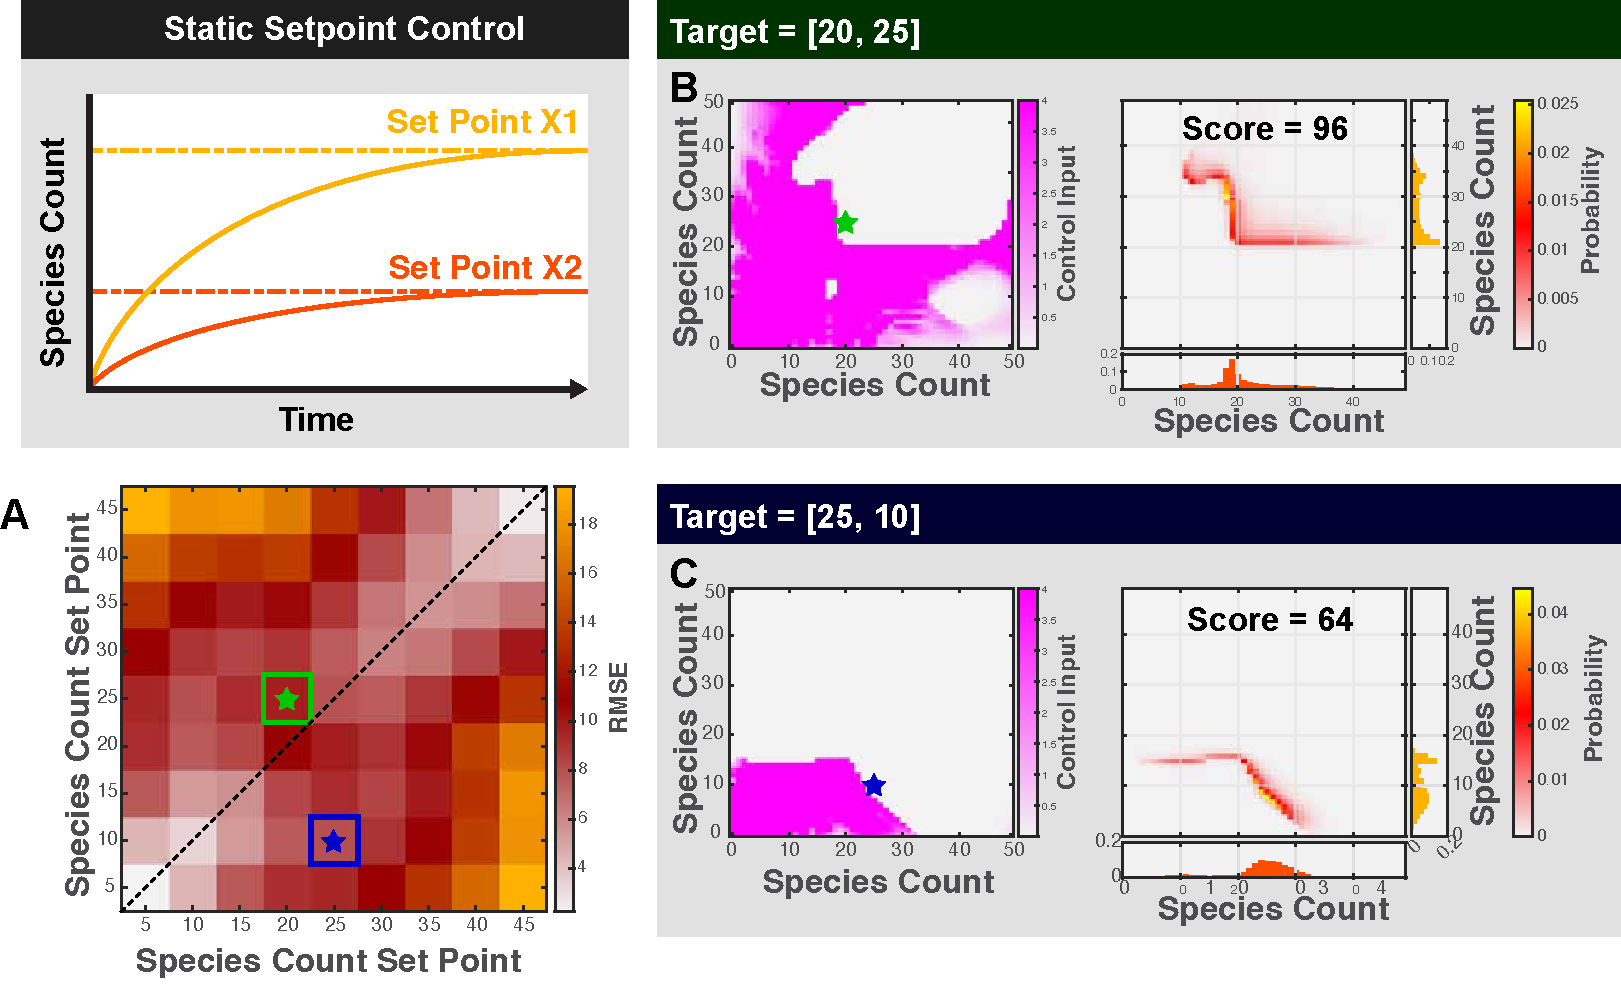
\includegraphics[width=1\textwidth]{ControlPoints.pdf}
\vspace{-0.1in}
\caption{Controllers optimized to a 2d domain of target points (A) show good control performance in the central region despite a broad range of targets (B and C). }
\label{CtrlP}
\end{center}
\vspace{-0.2in}
\end{figure*}

Many controllers were optimized to different target points to determine if certain reference points were harder to control than others. Controllers were optimized over a two dimensional domain of target points $(T_1,T_2)$between between five and fourty-five. Figure \ref{CtrlP} (A) shows the control performance of the system after optimizing each controller to each point in the domain. Figure \ref{CtrlP} (B and C) show the optimized control input and the steady state of two points in the system. The unstable point in the rate equation matches the unstable point near $(20,20)$ in this domain.

\begin{figure*}
\begin{center}
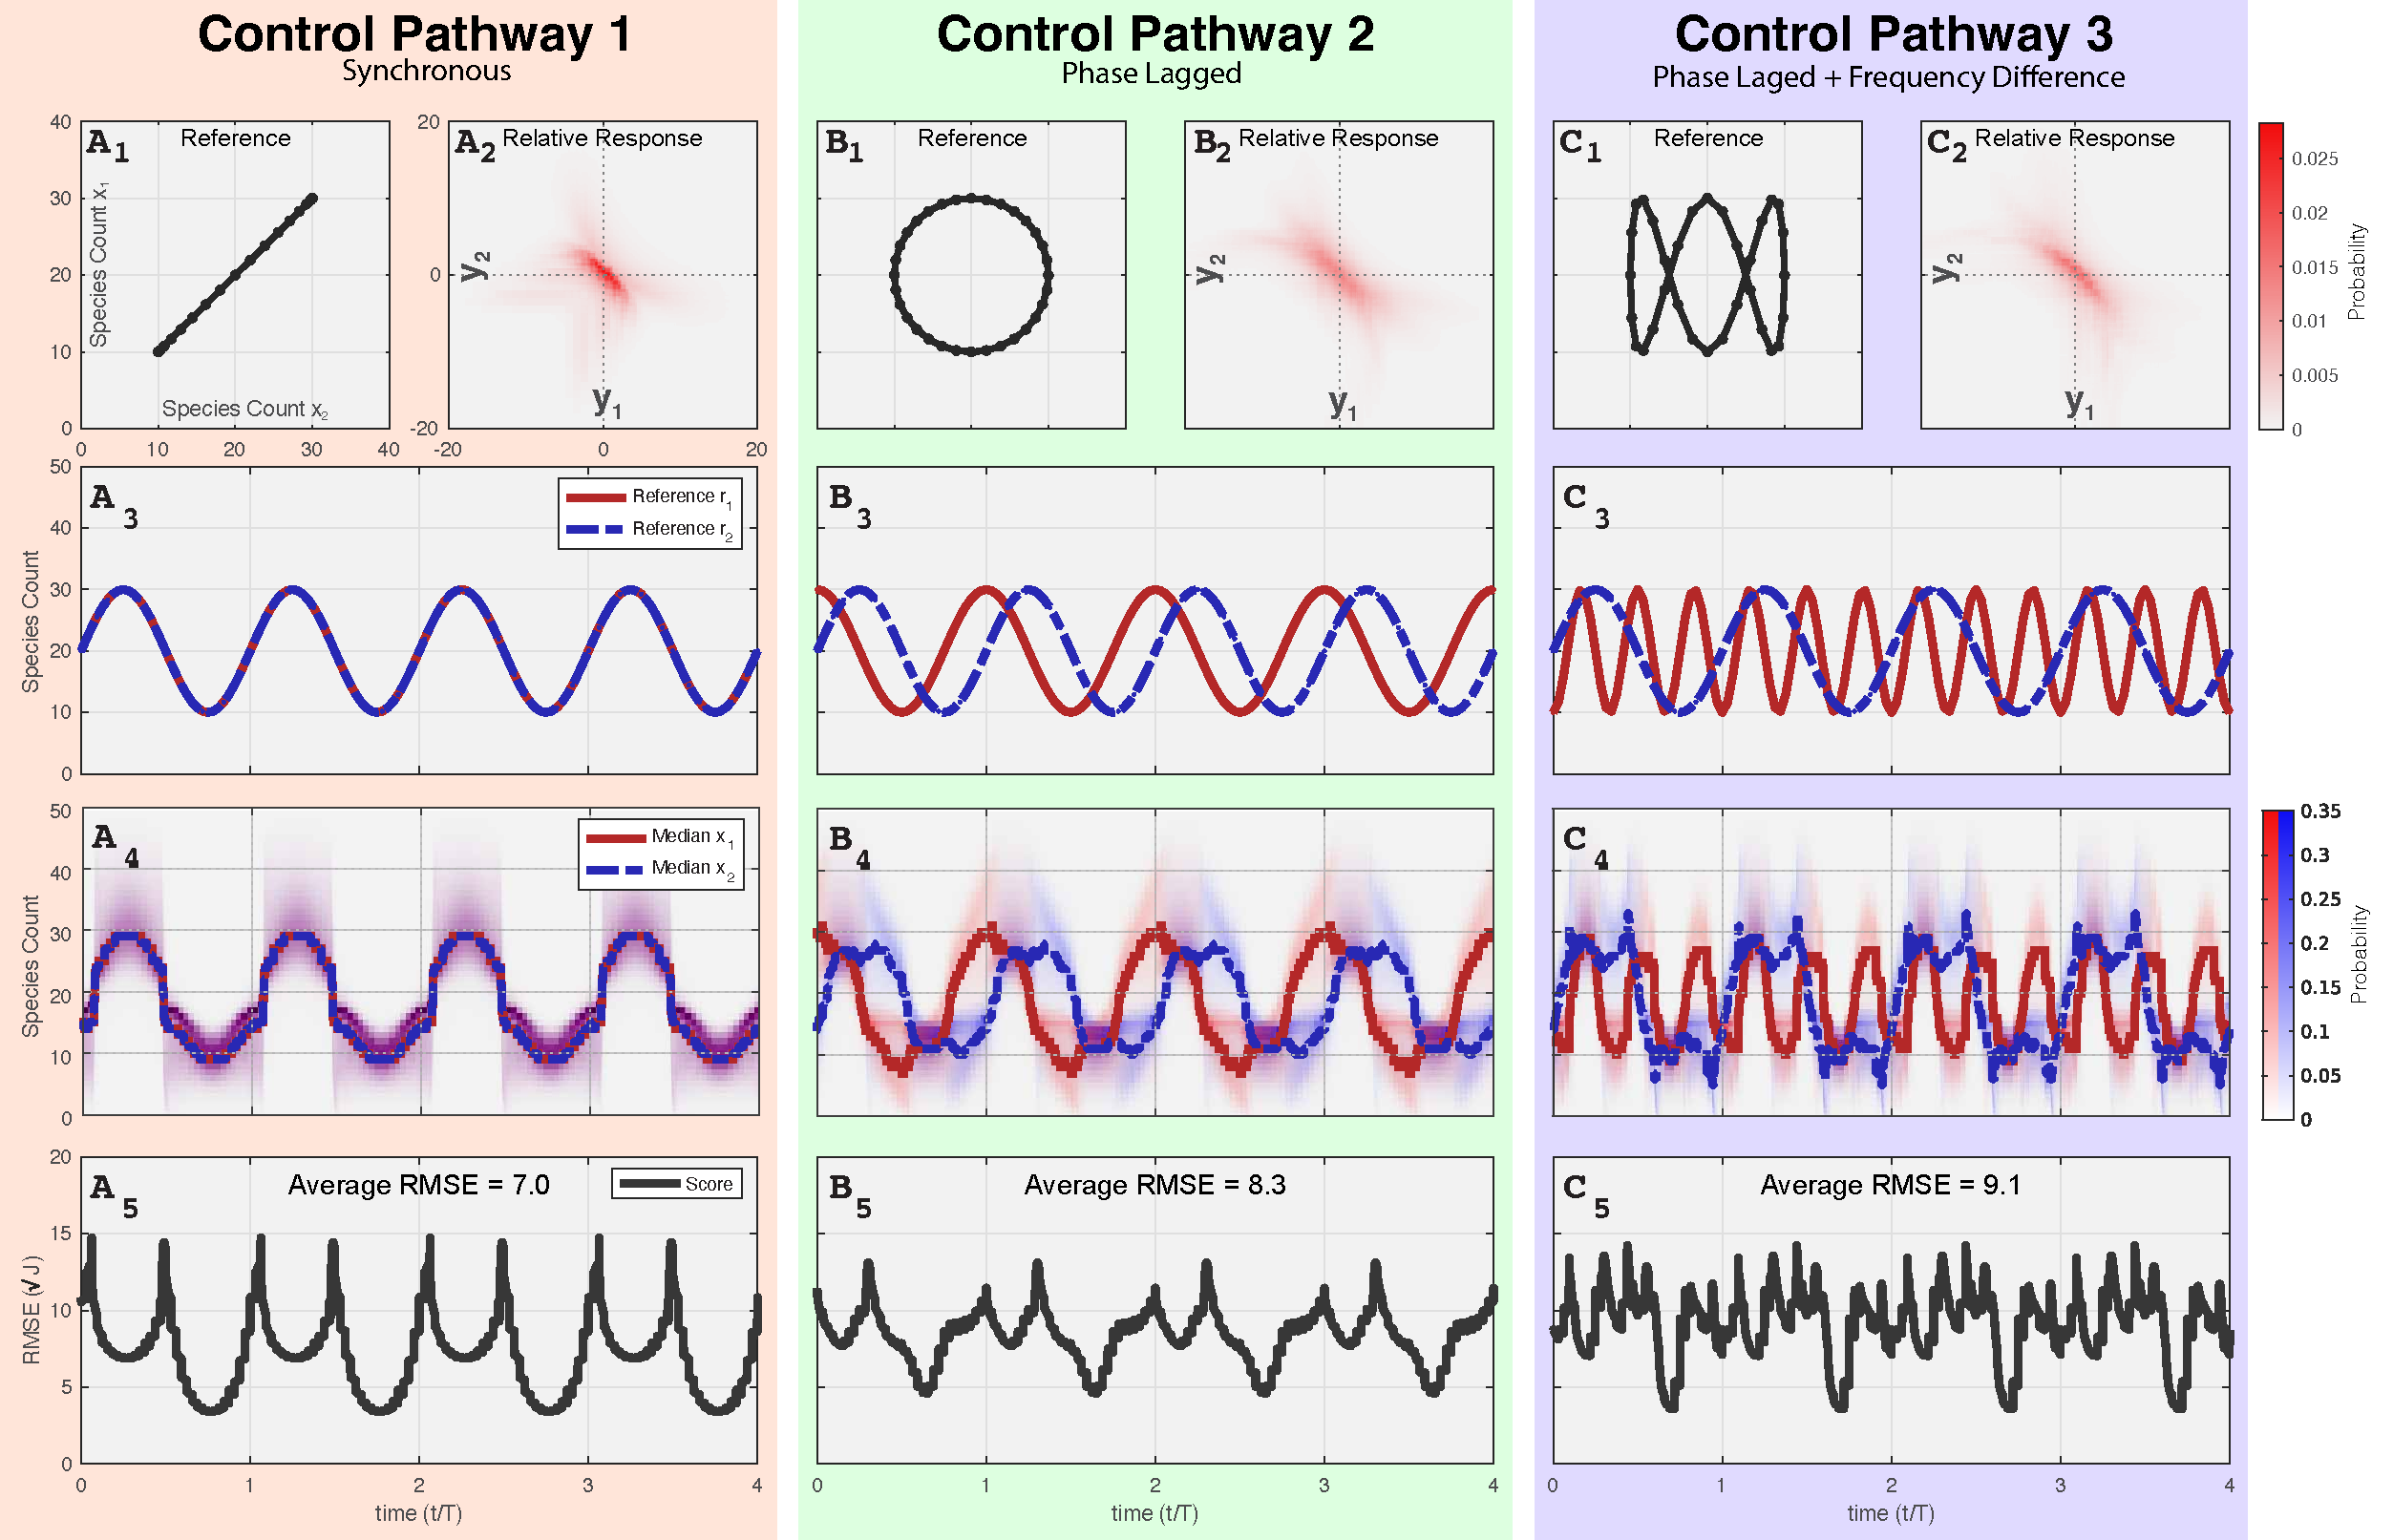
\includegraphics[width=1\textwidth]{ControlReference.pdf}
\vspace{-0.1in}
\caption{Finite state projections of the slowly driven system demonstrate good control performance under a variety of phase and frequency scenario. }
\label{CR}
\end{center}
\vspace{-0.2in}
\end{figure*}

Dynamic reference targeting was performed by cycling though individual controllers which were optimized to a single target point at a fixed frequency. Thirty-two controllers were optimized along a pathway in order to target an in-sync reference point \ref{CR}(Synchronous), a phase lagged reference point \ref{CR}(Phase Lagged), or frequency separated reference point\ref{CR}(Phase Lagged and Frequency). 
The in phase signal is given by $r(t)=XXX$, the phase-lagged signal is given by $r(t)=XXX$, and the frequency driven signal is given by $r(t)=XXX$ FSP simulations of cyclically driven systems were slowly driven at a frequency of 1/5000 seconds and their medians are shown in the Fig \ref{CR}(A4, B4,C4)(red cloud, blue cloud). Root mean squared error of each simulation are shown in Fig \ref{CR}(A5, B5,C5). Simulations show that in-phase control performed the best with an RSME of $7.0$ despite moving over the unstable point in the system. When the system is driven with a phase-lag the RSME of the score increases to $8.3$ and when driven at a different frequency the RMSE goes up to $9.1$. 


\begin{figure*}
\begin{center}
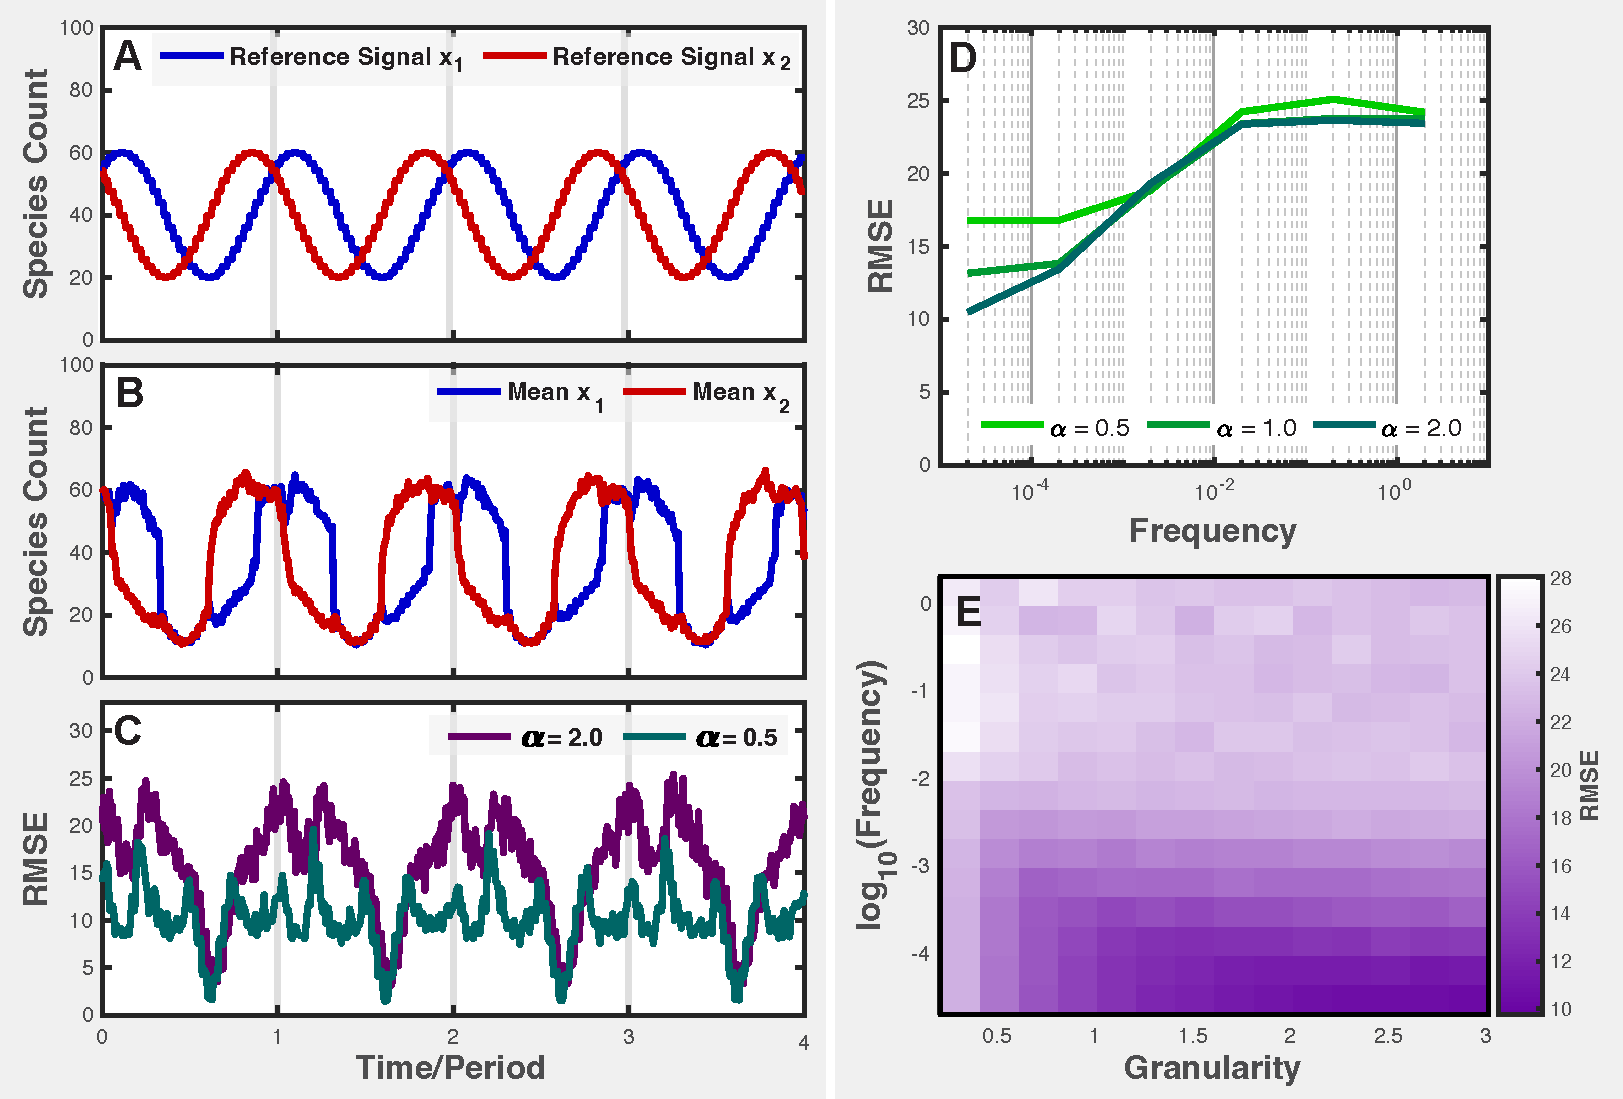
\includegraphics[width=1\textwidth]{ControlGranularityAndFrequency.pdf}
\vspace{-0.1in}
\caption{Stochastic simulations driven using a phased lagged controller show improved score at high granularity and low frequency.}
\label{CRG}
\end{center}
\vspace{-0.2in}
\end{figure*}
Although the control of a dynamic reference point using a Piecewise controller is possible, the effect of cycling frequency is also important.

16 SSA simulations of the phase-separated driving controller were performed on a system over a two dimensional domain of points $(\alpha,f)$ for a time of XXX minutes. Comparisons of control performance at $\alpha=0.5$ and $\alpha=2.0$ (Fig (C))show that control performance improves with system scale. 16 SSA simulations of the high granularity system driven by phase-lag were performed over a range of frequency values.  These analysis show that at low frequency the systems have a noise floor which decreases with increasing alpha, but was the system were driven rapidly, all systems became equally uncontrollable. At high frequency, the scores never got worse than $J=650$. At high frequency the control performance plateaus, while at lower frequency the system improves with increasing $\alpha$ Fig(E).

\section{Conclusion}
Key results from \cite{May2021} showed that noise was a key requirement for the development of a noise-exploiting controller, and that deterministic systems could not be controlled to two different stable points if they both started at the same initial condition. As a stochastic system becomes increasingly more granular, it also becomes less noisy and more similar to its ODE solution which is known to be impossible to control to two different fates, but here, we have shown that the removal of noise through system granularity led to better control performance.  Therefore, stochastic controllers may perform work best on models which are nearly deterministic, but not quite. Unfortunately, such systems were found to take longer time to achieve steady state.

The ability to analyze the model at one system granularity apply it elsewhere might help analyze models for which the computational effort may be too large. Since the computation time of the FSP solution to the CME grows with the square of the number of states, this can cause an explosion in computational requirements for large systems. One alternative is to learn a controller at a computationally feasible number of states and apply them to large systems which cannot be solves for using the FSP. 

Parameter perturbation analysis showed that there is room to improve control performance by adjusting system parameters, and that joint optimization of the controller with the system parameters may lead to better control performance. It also shows that populations of cells where each cell might have its own parameter combination could still be reasonably controlled for small changes in parameter scale, but large changes could be detrimental.

Time delay analysis showed that increasing time delay decreased control performance. It was also found that a controller with less control information outperformed a controller with more information at higher levels of time delay. We believe this is happening because a controller with more information can afford to be more aggressive to implement its control, and time delay can cause this aggression to backfire. A controller was optimized which required no information in May et al which had a score of 402. This controller should be immune to time delay since no feedback is required for this controller. Here we saw both controllers did performed worse than 402 at very large time delay.


\begin{thebibliography}{10}
\providecommand{\url}[1]{#1}
\csname url@samestyle\endcsname
\providecommand{\newblock}{\relax}
\providecommand{\bibinfo}[2]{#2}
\providecommand{\BIBentrySTDinterwordspacing}{\spaceskip=0pt\relax}
\providecommand{\BIBentryALTinterwordstretchfactor}{4}
\providecommand{\BIBentryALTinterwordspacing}{\spaceskip=\fontdimen2\font plus
\BIBentryALTinterwordstretchfactor\fontdimen3\font minus
  \fontdimen4\font\relax}
\providecommand{\BIBforeignlanguage}[2]{{%
\expandafter\ifx\csname l@#1\endcsname\relax
\typeout{** WARNING: IEEEtran.bst: No hyphenation pattern has been}%
\typeout{** loaded for the language `#1'. Using the pattern for}%
\typeout{** the default language instead.}%
\else
\language=\csname l@#1\endcsname
\fi
#2}}
\providecommand{\BIBdecl}{\relax}
\BIBdecl

\bibitem{May2021}
M.~May and B.~Munsky, ``{Exploiting noise, nonlinearity, and feedback to
  differentially control multiple synthetic cells with a single optogenetic
  input},'' pp. 1--28, 2021.
eps
\bibitem{Ng2019}
A.~H. Ng, T.~H. Nguyen, M.~G{\'{o}}mez-Schiavon, G.~Dods, R.~A. Langan, S.~E.
  Boyken, J.~A. Samson, L.~M. Waldburger, J.~E. Dueber, D.~Baker, and
  H.~El-Samad, ``{Modular and tunable biological feedback control using a de
  novo protein switch},'' pp. 265--269, 2019.

\bibitem{Liu2018}
C.~C. Liu, M.~C. Jewett, J.~W. Chin, and C.~A. Voigt, ``{Toward an orthogonal
  central dogma},'' \emph{Nature Chemical Biology}, vol.~14, no.~2, pp.
  103--106, 2018.

\bibitem{Sheets2020}
M.~B. Sheets, W.~W. Wong, and M.~J. Dunlop, ``{Light-Inducible Recombinases for
  Bacterial Optogenetics},'' \emph{ACS Synthetic Biology}, vol.~9, no.~2, pp.
  227--235, 2020.

\bibitem{Groseclose2020}
\BIBentryALTinterwordspacing
T.~M. Groseclose, R.~E. Rondon, Z.~D. Herde, C.~A. Aldrete, and C.~J. Wilson,
  ``{Engineered systems of inducible anti-repressors for the next generation of
  biological programming},'' \emph{Nature Communications}, vol.~11, no.~1, pp.
  1--15, 2020. [Online]. Available:
  \url{http://dx.doi.org/10.1038/s41467-020-18302-1}
\BIBentrySTDinterwordspacing

\bibitem{Shin2020}
J.~Shin, S.~Zhang, B.~S. Der, A.~A. Nielsen, and C.~A. Voigt, ``{ Programming
  Escherichia coli to function as a digital display },'' \emph{Molecular
  Systems Biology}, vol.~16, no.~3, pp. 1--12, 2020.

\bibitem{Baumschlager2017}
A.~Baumschlager, S.~K. Aoki, and M.~Khammash, ``{Dynamic blue light-inducible
  T7 RNA polymerases (Opto-T7RNAPs) for precise spatiotemporal gene expression
  control},'' \emph{ACS synthetic biology}, vol.~6, no.~11, pp. 2157--2167,
  2017.

\bibitem{Chen2020}
\BIBentryALTinterwordspacing
S.~Y. Chen, L.~C. Osimiri, M.~Chevalier, L.~J. Bugaj, T.~H. Nguyen, R.~A.
  Greenstein, A.~H. Ng, J.~Stewart-Ornstein, L.~T. Neves, and H.~El-Samad,
  ``{Optogenetic Control Reveals Differential Promoter Interpretation of
  Transcription Factor Nuclear Translocation Dynamics},'' \emph{Cell Systems},
  vol.~11, no.~4, pp. 336----353.e24, 2020. [Online]. Available:
  \url{http://dx.doi.org/10.1016/j.cels.2020.08.009}
\BIBentrySTDinterwordspacing

\bibitem{Lillacci2018}
G.~Lillacci, Y.~Benenson, and M.~Khammash, ``{Synthetic control systems for
  high performance gene expression in mammalian cells},'' \emph{Nucleic acids
  research}, vol.~46, no.~18, pp. 9855--9863, 2018.

\bibitem{Fox2021}
\BIBentryALTinterwordspacing
Z.~R. Fox, S.~Fletcher, A.~Fraisse, C.~Aditya, and S.~Sosa, ``{MicroMator: Open
  and Flexible Software for Reactive Microscopy},'' \emph{bioRxiv}, pp. 1--9,
  2021. [Online]. Available:
  \url{http://biorxiv.org/cgi/content/short/2021.03.12.435206v1}
\BIBentrySTDinterwordspacing

\bibitem{Baumschlager2021}
\BIBentryALTinterwordspacing
A.~Baumschlager and M.~Khammash, ``{Synthetic Biological Approaches for
  Optogenetics and Tools for Transcriptional Light-Control in Bacteria},''
  \emph{Advanced Biology}, vol.~5, no.~5, p. 2000256, 2021. [Online].
  Available:
  \url{https://onlinelibrary.wiley.com/doi/abs/10.1002/adbi.202000256}
\BIBentrySTDinterwordspacing

\bibitem{Lugagne2017}
\BIBentryALTinterwordspacing
J.~B. Lugagne, S.~{Sosa Carrillo}, M.~Kirch, A.~K{\"{o}}hler, G.~Batt, and
  P.~Hersen, ``{Balancing a genetic toggle switch by real-time feedback control
  and periodic forcing},'' \emph{Nature Communications}, vol.~8, no.~1, pp.
  1--7, 2017. [Online]. Available:
  \url{http://dx.doi.org/10.1038/s41467-017-01498-0}
\BIBentrySTDinterwordspacing

\bibitem{Rullan2018}
\BIBentryALTinterwordspacing
M.~Rullan, D.~Benzinger, G.~W. Schmidt, A.~Milias-Argeitis, and M.~Khammash,
  ``{An Optogenetic Platform for Real-Time, Single-Cell Interrogation of
  Stochastic Transcriptional Regulation},'' \emph{Molecular Cell}, vol.~70,
  no.~4, pp. 745--756.e6, 2018. [Online]. Available:
  \url{https://doi.org/10.1016/j.molcel.2018.04.012}
\BIBentrySTDinterwordspacing

\bibitem{Guarino2020}
A.~Guarino, D.~Fiore, D.~Salzano, and M.~{Di Bernardo}, ``{Balancing Cell
  Populations Endowed with a Synthetic Toggle Switch via Adaptive Pulsatile
  Feedback Control},'' \emph{ACS Synthetic Biology}, vol.~9, no.~4, pp.
  793--803, 2020.

\bibitem{Munsky2012}
B.~Munsky, G.~Neuert, and A.~Van~Oudenaarden, ``{Using gene expression noise to
  understand gene regulation},'' \emph{Science}, vol. 336, no. 6078, pp.
  183--187, 2012.

\bibitem{Szymanska2015}
P.~Szyma{\'{n}}ska, N.~Gritti, J.~M. Keegstra, M.~Soltani, and B.~Munsky,
  ``{Using noise to control heterogeneity of isogenic populations in homogenous
  environments},'' \emph{Physical Biology}, vol.~12, no.~4, 2015.

\bibitem{Gillespie1992}
D.~T. Gillespie, ``{A rigorous derivation of the chemical master equation},''
  \emph{Physica A: Statistical Mechanics and its Applications}, vol. 188, no.
  1-3, pp. 404--425, 1992.

\bibitem{Gillespie1977}
D.~T. Gillespie, ``{Exact stochastic simulation of coupled chemical reactions},''
  \emph{The journal of physical chemistry}, vol.~81, no.~25, pp. 2340--2361,
  1977.

\end{thebibliography}

\end{document}

